\documentclass[a4paper,oneside]{mystyle}
\usepackage[utf8]{inputenc}

% custom packages
\usepackage{empheq}
\usepackage{graphicx}
\usepackage[font={small}]{caption}
\usepackage{subcaption}
\usepackage{framed}
\usepackage{listings}
\usepackage{wrapfig}
\usepackage{sidecap}
\usepackage{xcolor}
\usepackage{lineno}
\usepackage{marvosym}
\usepackage{xstring}
\usepackage{mfirstuc}
\usepackage{pdfpages}
\usepackage{lipsum}
\usepackage{lettrine}
\usepackage[explicit]{titlesec}
\usepackage{cancel}
\usepackage[noabbrev]{cleveref}
\usepackage{indentfirst}
\usepackage{mathtools}
\usepackage{algorithmicx}
\usepackage{algpseudocode}
\usepackage{algorithm}
\usepackage{hyperref}
\usepackage{nicefrac}


%%%%%%%%%%%%%%%%%%%%%%%%%%%%%%%%%%%%%%%%%%%%%%%%%%%%%%%%%%%%%%%%%%%%%
% DOCUMENT METADATA

\thesistype{Master thesis}
\title{ProSLAM student edition: a minimalistic stereo visual SLAM system}

\author{Irvin Aloise}
\email{aloise.1392066@studenti.uniroma1.it}
\institute{RoCoCo - Cognitive robot teams laboratory\\[2pt]
Department of Computer, Control and Management Engineering Antonio Ruberti\\[2pt]
Sapienza University of Rome}

\supervisors{Prof.\ Dr.\ Giorgio Grisetti}
\cosupervisors{Eng.\ Dominik Schlegel}

\date{\today}

%%%%%%%%%%%%%%%%%%%%%%%%%%%%%%%%%%%%%%%%%%%%%%%%%%%%
\lstset { %
	language=C++,
	backgroundcolor=\color{black!5}, % set backgroundcolor
	basicstyle=\footnotesize,% basic font setting
}


%ds colors
\definecolor{orange}{rgb}{1,0.4,0}
\definecolor{green}{rgb}{0,0.5,0}

%ds referencing
\newcommand{\myref}[3]{\hyperref[#1]{#2} (\capitalisewords{#3} \ref{#1})}

%ds blue box
\definecolor{myblue}{rgb}{.9, .9, 1}

\newlength\mytemplen
\newsavebox\mytempbox
\newcommand*\widefbox[1]{\fbox{\hspace{2em}#1\hspace{2em}}}

\makeatletter
\newcommand\mybluebox{%
	\@ifnextchar[%]
	{\@mybluebox}%
	{\@mybluebox[0pt]}}

\def\@mybluebox[#1]{%
	\@ifnextchar[%]
	{\@@mybluebox[#1]}%
	{\@@mybluebox[#1][0pt]}}

\def\@@mybluebox[#1][#2]#3{
	\sbox\mytempbox{#3}%
	\mytemplen\ht\mytempbox
	\advance\mytemplen #1\relax
	\ht\mytempbox\mytemplen
	\mytemplen\dp\mytempbox
	\advance\mytemplen #2\relax
	\dp\mytempbox\mytemplen
	\colorbox{myblue}{\hspace{1em}\usebox{\mytempbox}\hspace{1em}}}

%ds global definitions
\def\zero{\mathbf{0}}
\def\P{\mathcal P}
\def\tab{\phantom{tab}}
\def\homx{\mathbf{\tilde{x}}}
\def\trans{\mathbf{t}}
\def\quat{\mathbf{q}}
\def\state{\mathbf{x}}
\def\SState{\mathbf{X}}
\def\meas{\mathbf{z}}
\def\tmeas{\tilde{\meas}}
\def\Meas{\mathbf{Z}}
\def\pred{\hat{\meas}}
\def\linstate{\breve{\state}}
\def\Linstate{\breve{\SState}}
\def\optstate{\state^\star}
\def\Optstate{\State^\star}
\def\dx{\Delta \state}
\def\dz{\Delta \meas}
\def\hessian{\mathbf{H}}
\def\bvec{\mathbf{b}}
\def\error{\mathbf{e}}
\def\terror{\tilde{\error}}
\def\jacob{\mathbf{J}}
\def\tjacob{\tilde{\jacob}}
\def\kdtree{\textit{K}-D tree}
\def\T#1#2{^{#1}T_{#2}}
\def\rot{\mathbf{R}}
\def\t2v#1#2{^{#1}\tau_{#2}}
\def\deltat2v#1#2{^{#1}\Delta\tau_{#2}}
\def\chref#1{Chapter~\ref{ch:#1}}
\def\secref#1{Sec.~\ref{#1}}
\def\figref#1{Fig.~\ref{#1}}
\def\tabref#1{Tab.~\ref{#1}}
\def\eqref#1{Eq.~(\ref{#1})}
\def\algref#1{Alg.~\ref{#1}}
\def\lstref#1{Lst.~\ref{#1}}
\def\ourmethod{\textit{g2o\_slim~}}
\renewcommand{\thesubfigure}{\Alph{subfigure}}

% mathemagical stuff
\DeclareMathOperator*{\argmax}{argmax}
\DeclareMathOperator*{\argmin}{argmin}
\newcommand{\pluseq}{\mathrel{+}=}
\newcommand{\asteq}{\mathrel{*}=}

% indentation stuff
\newlength\myindent
\setlength\myindent{2em}
\newcommand\bindent{%
    \begingroup
    \setlength{\itemindent}{\myindent}
    \addtolength{\algorithmicindent}{\myindent}
}
\newcommand\eindent{\endgroup}

\begin{document}
	
\frontmatter
\begin{titlepage}
\maketitle
\cleardoublepage\null
\thispagestyle{empty}
\end{titlepage}

\newcounter{notation}
\begin{abstract}
The goal of this Master's Thesis is the design and development of a graph-optimization system tailored for SLAM pipelines. The work focuses on simplicity, accuracy and speed, reaching excellent results in each of the targeted fields.

In particular, this back-end aims attention at 3D pose-graphs and 3D pose-landmark problems, producing outcomes comparable to current state-of-the-art systems like \texttt{g2o} \cite{kummerle2011g}. 

At its core there is a novel error function for $SE(3)$ objects based on the concept of matrices' chordal distance. This approach reduces the problem's non-linearity bringing several benefits to the computation. The fastness of the system is due to a well-designed implementation that performs zero memory copy during the iterative part and that exploits SIMD instructions of modern CPUs and a smart use of the CPU cache.

Finally, the system has been tested on both synthetic and real-world datasets and in both scenarios it succeeded in its purposes, being able to produce results better or comparable to state-of-the-art systems in only 5 thousands lines of code. 
\end{abstract}

\chapter*{Nomenclature}\label{ch:symbols}
\addcontentsline{toc}{chapter}{Nomenclature}

\section*{Notation}
\refstepcounter{notation}
\label{sec:notation}

\begin{tabbing}
	\hspace*{3.0cm}		\= \kill
	$^A\rot_{B}(\alpha, \beta, \gamma)$ \> Rotation from frame A to frame B expressed in A \\[0.75ex]
	$^A\trans_{B}(t_x,t_y,t_z)$ \> Translation from frame A to frame B expressed in A  \\[0.75ex]
	$\T{A}{B}(R,\trans)$ \> Transformation from frame A to B expressed in A  \\[0.75ex]
	$\t2v{A}{B}(R,\trans)$ \> Transformation from frame A to B expressed in A (vectorized) \\[0.75ex]
	${\lfloor\trans\rfloor}_\times$ \> Skew-symmetric matrix of a vector $\mathbf{t} \in \mathbb{R}^{3\times3}$
\end{tabbing}

\section*{Acronyms and Abbreviations}
\label{sec:acronyms}
\begin{tabbing}
	\hspace*{3.5cm}		\= \kill
	SLAM \> Simultaneous localization and mapping \\[1ex]
    SfM \> Structure from Motion \\[1ex]
    BA \> Bundle Adjustment \\[1ex]
    SCLAM \> Simultaneous Calibration Localization and Mapping \\[1ex]
    MAP \> Maximum A Posteriori \\[1ex]
    LS \> Least Squares \\[1ex]
    PSD \> Positive Semi-Definite \\[1ex]
    PDF \> Probability Distribution Function \\[1ex]
    Landmark \> Salient point in the world (2D or 3D) \\[1ex]
	Feature \> Specific structural part of interest in an image (2D) \\[1ex]
	Tracking \> Procedure of spatial and temporal re-identification of landmarks \\[1ex]
	Loop closure \> Interconnection between landmarks in space \\[1ex]
	GPS \> Global Positioning System (generally referring to whole unit) \\[1ex]
    LiDAR \> Light Detection and Ranging o Laser Imaging Detection and Ranging \\[1ex]
    Sonar \> SOund Navigation And Ranging \\[1ex]
    FLOP \> Floating Point OPeration \\[1ex]
    FLOPS \> Floating Point Operations Per Second \\[1ex]
	OpenCV  \> Open source Computer Vision (library), \url{www.opencv.org} \\[1ex]
	Git  \> Git revision control, \url{www.git-scm.com} \\[1ex]
\end{tabbing}

\clearpage

\tableofcontents
\mainmatter
\newpage
\chapter{Introduction}\label{ch:intro}
Mobile robots, in order to accomplish tasks in real world more easily and in an efficient way, need to have a map of the environment and to localize themselves into the map. Furthermore, in some environment it is not possible to rely on external reference systems - e.g. GPS - and, thus, they can count only on on-board sensors. \textit{Simultaneous Localization and Mapping} (SLAM) addresses the problem of \textbf{learning the map under pose uncertainty}.

There are many scenarios in which SLAM is fundamental for the accomplishment of a task, not only in pure Robotics. SLAM, in fact, is a common problem in different domains of application. For example, in Robotics it is fundamental for indoor navigation of mobile robots - e.g. an autonomous vacuum cleaner or a service robot in a museum - or to navigate through extreme environments - e.g. underwater rescues or space exploration. Additionally, new technologies that involve different kind of agents - i.e. not robots - are now using SLAM. One of the most trending is \textit{Augmented Reality} (AR). Always more powerful mobile devices - like smartphones or tablets - are now able to exploit SLAM to deliver stunning virtual experiences. Without any doubts, this technology is going to gain always more popularity and to impact on the research in this topic.
\vspace{5px}

\begin{figure}[!hbt]
    \centering
    \begin{minipage}[t!]{0.4\textwidth}
        \centering
        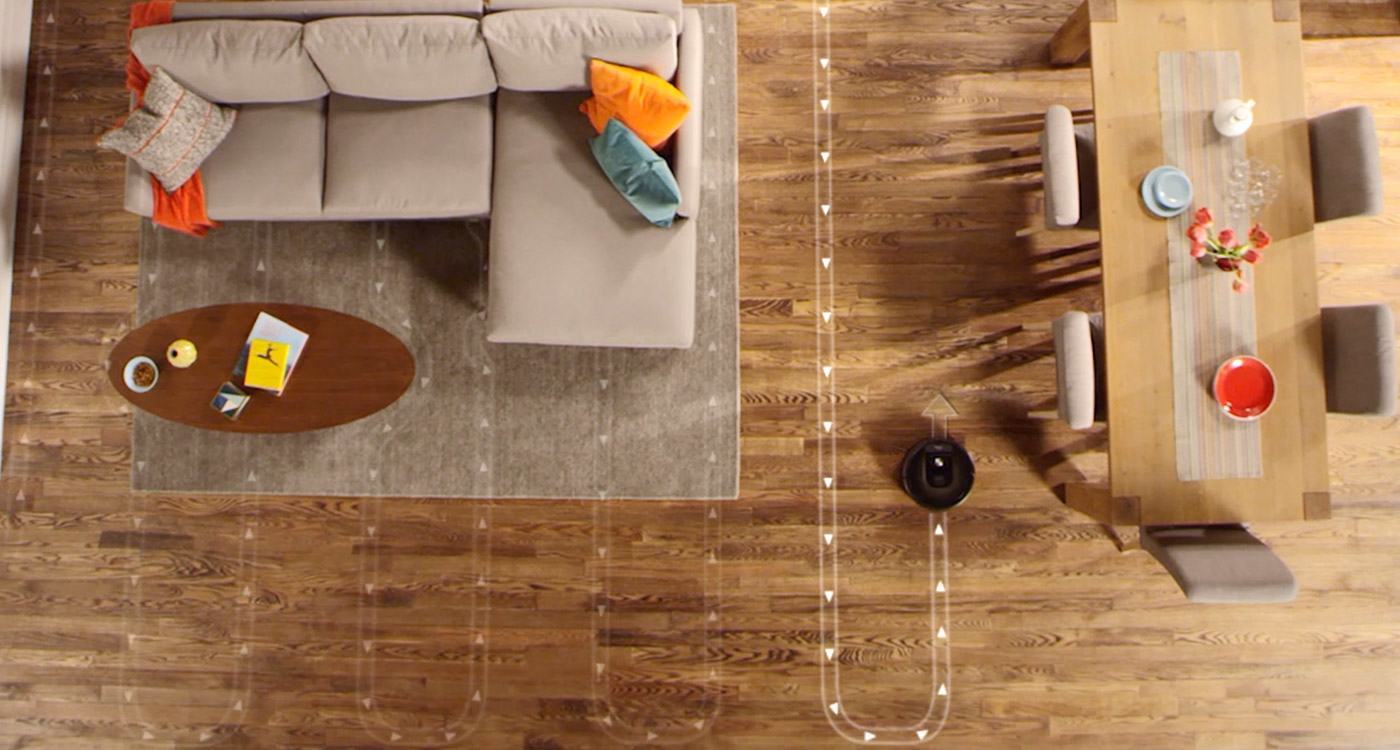
\includegraphics[width=\textwidth]{figures/00_intro/roomba_cleaning.jpg}
        \subcaption[first caption.]{}
        \label{fig:roomba}
    \end{minipage} \hspace{10px}
    \begin{minipage}[t!]{0.4\textwidth}
        \centering
        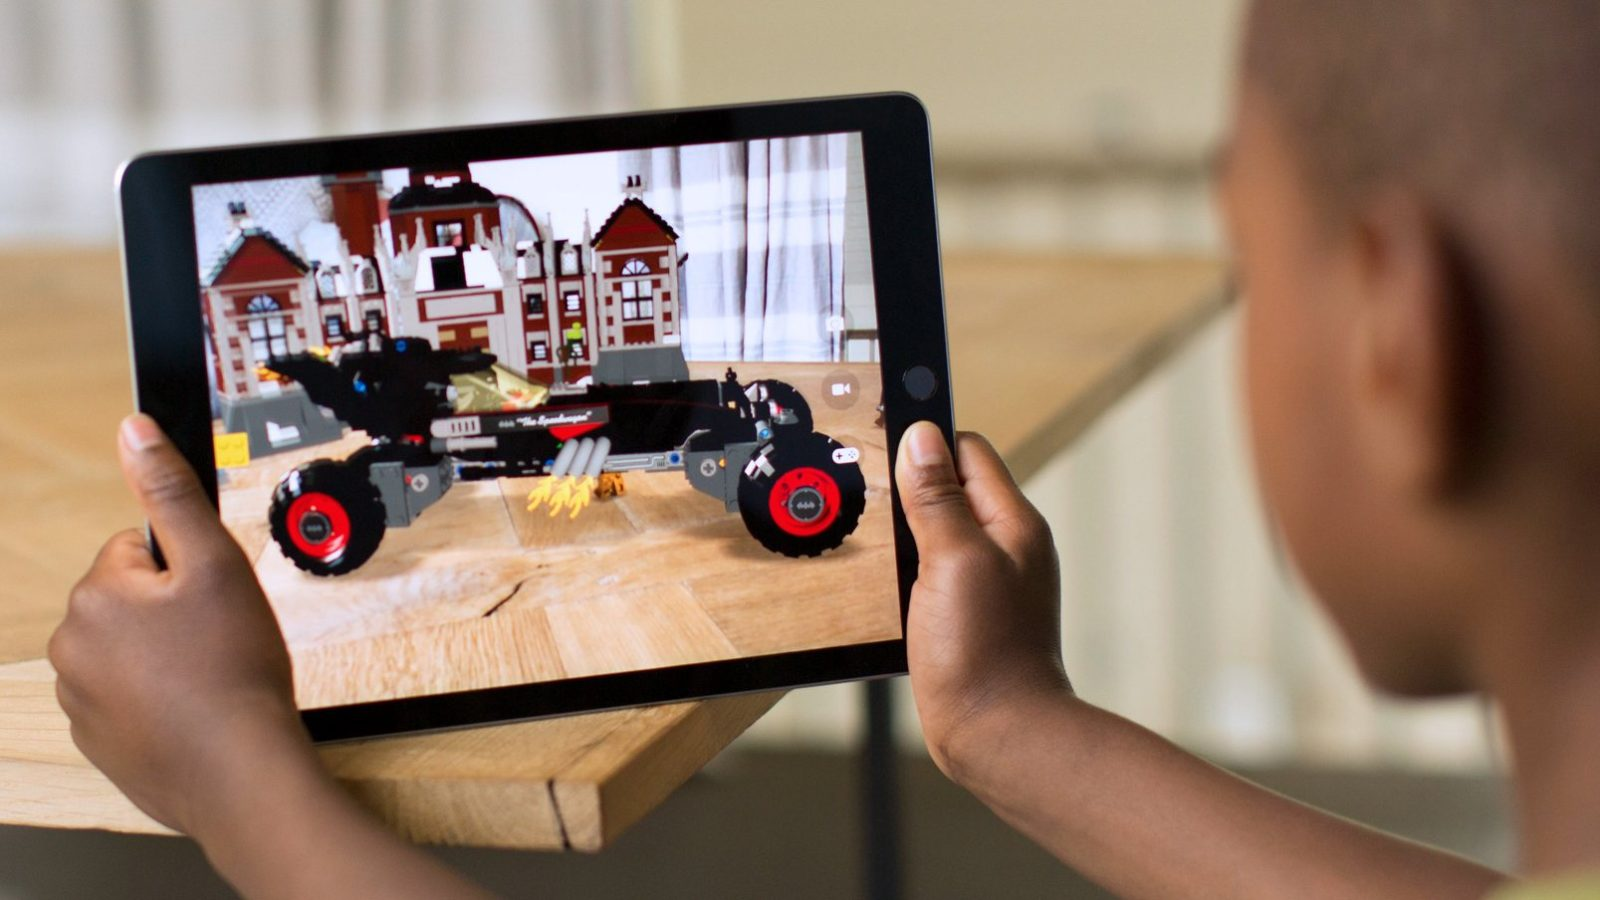
\includegraphics[width=\textwidth]{figures/00_intro/apple_ARKit.jpg}
        \subcaption[second caption.]{}
        \label{fig:apple_ARKit}
    \end{minipage}%
    
    \caption{\textbf{Application Examples.} The image in \ref{fig:roomba} represents the well-known Roomba Autonomous vacuum cleaner, which is able to recognize where it is in the room, if it has already cleaned a place or if it is going toward a dangerous path - e.g. stairs; image \ref{fig:apple_ARKit} depicts an AR mobile game developed using the Apple ARKit.} 
    \label{fig:applications}
\end{figure}

As the reader might notice, SLAM is a popular problem and the research community is focusing on it since many years. Several solutions have been proposed through the years and now current state-of-the-art SLAM systems are able to deliver impressive results in real-world scenarios. The most used formulation for the SLAM problem is the so-called \textit{graph-based SLAM}. In this approach, two sub-systems cooperate with each other to retrieve the best robot trajectory and world configuration given the on-board sensors' measurements. Therefore, the full slam system is composed by:

\begin{enumerate}
    \item \textit{Front-end}: it exploits sensor data to build an hyper-graph whose nodes are either robot poses or the position of salient points in the world;
    \item \textit{Back-end}: it is in charge of performing non-linear optimization of the graph to retrieve the most likely configuration that suits the measurements.
\end{enumerate}

In this work, we propose a back-end system built from scratch that is able to perform fast and accurate graph optimization for 3D environments. The work is focused on simplicity and minimalism also in its implementation, in order to be comprehensible by non-expert people that what to understand how the system works. Despite its minimalistic fashion, system's results are comparable - or even better in some scenarios - to the ones of other state-of-the-art systems, thanks to the use of some novel theoretic ideas and to a well-designed implementation. In particular, this work shows the effectiveness of a \textbf{new error function} for $SE(3)$ objects (Section \ref{sec:se3_objects}) and an implementation with \textbf{zero memory copy} during the optimization process (Section \ref{sec:bottlenecks}).

\vspace{20px}

\noindent The remaining of this document is organized as follows:

\begin{itemize}
    \item Chapter \ref{ch:related}: overview of the problem and of methodologies employed through the years, with a particular focus on noteworthy systems;
    \item Chapter \ref{ch:basics}: problem statement and fundamental theoretic concepts related to the non-linear optimization problem;
    \item Chapter \ref{ch:problems}: sketch of the most common SLAM problem formulations;
    \item Chapter \ref{ch:solvingSE3}: deeper examination of 3D formulations and further analysis of the proposed approach;
    \item Chapter \ref{ch:implementation}: details about code design and implementation choices;
    \item Chapter \ref{ch:cases}: focus on two full SLAM systems that uses the proposed system as on-line back-end;
    \item Chapter \ref{ch:conclusions}: final considerations and possible future investigations. 
\end{itemize}
\newpage
\chapter{Related Works}\label{ch:related}
Simultaneous Localization and Mapping represents a well known complex mathematical problem, based on non-linear optimization. It has been studied by the robotics community since the 80s \cite{durrant2006simultaneous} \cite{bailey2006simultaneous}; during this early stage, its statistical formulation has been investigated, proposing interesting results that will constitute the baseline basically for all the future SLAM systems.

After some years, in the 90s, early solutions to the SLAM problem start to arise. The first systems able to produce appreciable results in terms of speed and accuracy were based on \textit{Extended Kalman Filters} (EKF) \cite{leonard1990dynamic} \cite{dissanayake2001solution}. EKFs allow to deal with problem's non-linearity through effective approximations and to represent multivariate distributions with a small number of parameters. This success encouraged the research community to perform deeper investigations in \textit{filtering} approaches \cite{aulinas2008filtering_review}. \textit{Particle filters} started to gain popularity, in particular \textit{Rao-Blackwellized Particle Filters} \cite{grisetti2005improving}: the work of Montemerlo \textit{et al.} \cite{montemerlo2002fastslam} was the first SLAM system able to deal with thousand of landmarks with a good accuracy. 

However, \textit{filtering} approaches revealed to be not the best answer to the SLAM problem due to the computational complexity of the solution, especially when dimensions grow. Moreover, system's accuracy is affected by the non-linearities, leading to non-optimal solutions. \textit{Maximum A Posteriori} (MAP) starts to be taken in consideration and the community has taken a step back to the work of Lu \textit{et al.} \cite{lu1997globally}. Filtering-based approaches align local pose frames incrementally and, thus, different parts of the model are updated independently, generating inconsistencies in the model. MAP optimization takes in consideration all the local frames and the relations between them at once, leading to a more consistent model and to better accuracy. Lu \textit{et al.} embedded all the pose relations into an network with nodes and edges, allowing efficient optimization. However, at that time the computational power was not enough to deliver good performance and, thus, this solution was put aside.

Nevertheless, this work represents the precursor to one the most intuitive SLAM formulation, called \textit{graph-based SLAM}, that exploits the computing power of recent robots to deliver impressive performances. In this paradigm, the robot builds an \textit{hyper-graph} whose nodes represents either robot poses or salient points in the world - called \textit{landmarks} - while the hyper-edges encode sensors' measurements between subsets of nodes. 

Graph-based SLAM systems have two main components: \textit{front-end} and \textit{back-end}. The former one uses data acquired by robot's sensors to populate the hyper-graph, abstracting raw data into a model that is amenable for optimization. The front-end has to determine the most likely constraint that involves a subset of nodes given an incoming measurement, solving the so called \textit{data association} problem. This includes \textit{short-term data association} and \textit{long-term} one. The former has to match corresponding extracted features with consecutive sensor measurements - e.g. stating that visual features detected in multiple consecutive frames represent the same 3D world point. The latter one, instead, expresses a more complex problem: it has to associate new measurements to already encountered world points, generating the so called \textit{loop-closures} - e.g. when a robot passes multiple times in a place, it has to recognize that it is re-observing the same points in order to generate a map that is consistent with the environment. As for the sensors used, state-of-the-art systems usually acquire data from cameras (RGB or RDB-D) or 3D-LiDARs. The former, in particular, it is gaining much attention since they are - generally - cheap and can be mounted basically on every electronic device in single or stereo configurations. 

This work, however, focuses on system's back-end, assuming that the given front-end provides consistent estimates. The back-end takes as input the graph and computes the most-likely map given all the constraints. Systems based on this formulation represent the gold standard for map optimization, thus, in the next sections it is proposed a brief overview of the most successful implementations.

\section{Dense Approaches}\label{sec:dense_approaches}
The work of Lu \textit{et al.} \cite{lu1997globally} was the first of its kind: map estimation is obtained through global optimization of the error function deriving from constraints between different poses. They employed a combination of \textit{relation-based} and \textit{location-based} representations, where the former were fixed while the latter were treated as free variables. Those pose-relations were used to construct a network whose nodes were robot poses taken from its trajectory while the constraints between nodes were the pose-relations. Finally, the optimization problem exploits the network to obtain an objective function that will be minimized: the total energy will decrease as the difference between estimated relative-pose that involves two nodes and the measured value tends to zero. 

It is good to notice that, in this formulation, the computational power needed for the optimization grow \textit{cubically} with the number of variables involved - graph's nodes. Gutmann and Konolige addressed this problem in their work \cite{gutmann1999incremental} proposing a method to incrementally build the network and that determines topologically correct relations between poses.

Those approaches opened the path to a series of study in this direction, that will lead to current state-of-the-art optimizers.

\section{Olson's Gradient Descent}\label{sec:olson}
Evident limitations of the previously seen approaches is that their solution highly depends from the initial estimate of the state. The initial guess is derived from dead-reckoning and, thus, if this is not good the system will converge to a local minimum, giving a sub-optimal solution. Olson \textit{et al.} proposed in their work \cite{olson2006fast} addressed this issue, proposing a non-linear optimization algorithm that quickly converges to a good approximation of the global minimum. 

They achieved such results combining two new aspects: the first one is the use of a variant of \textit{Stochastic Gradient Descent} algorithm, which is robust against local minima and has a fast convergence rate; the second one is an \textit{alternative state-space representation} that has good stability and computational properties. The latter, in particular, allows to update many poses with a relatively small computational cost in a single iteration. Moreover, the memory consumption has been lowered together with the run time - respectively $O(N + M)$ and $O(\log(N))$, where $N$ represents the number of poses and $M$ the number of constraints.

\section{Smoothing and Mapping}\label{sec:sam}
Smoothing and Mapping, shortened as \textit{SAM}, follows the path of global trajectory optimization described in the previous Section. Dellaert \textit{et al.} proposed with \textit{square root SAM} ($\sqrt{SAM}$) \cite{dellaert2006square} a system able to deal with \textit{full SLAM problems}, which involves estimating the entire set of sensor poses along with the parameters of all the features in the environment - also known in photogrammetry as \textit{bundle adjustment} and as \textit{structure from motion} in computer vision.

$\sqrt{SAM}$ performs fast optimization exploiting the problem's intrinsic sparsity. Knowing that the measurement Jacobian matrix $A$ is sparse, it is possible to solve the relative linear system in a faster way through a good \textit{variable reordering} together with \textit{QR} or \textit{Cholesky} factorization. For those reasons, $\sqrt{SAM}$ can optimize larger graph without losing in terms of performances or accuracy.

Further improvements were introduced with \textit{iSAM} - \textit{incremental} SAM - developed by Kaess \textit{et al.} \cite{kaess2007isam}. The foundations were the same as $\sqrt{SAM}$, but in this case the system operates incrementally, without the need of fully refactoring the whole QR-decomposition, but updating it every time a new measurement is available. With this solution, it was possible to address real-time problems since the optimization process is faster than before. 

The next iteration of this branch of solutions, is represented by \textit{iSAM2} \cite{kaess2012isam2}. In this case, a new data-structure is proposed, the \textit{Bayes tree}, to map better the square root information matrix of the problem. Employing Bayes trees, the algorithm is able to further improve the performances, exploiting incremental variable re-ordering and fluid relinearization, eliminating the need for periodic batch steps. 

\section{TORO}\label{sec:toro}
Grisetti \textit{et al.} proposed in their work TORO \cite{toro} - Tree-based netwORk Optimizer - an extension of Olson's algorithm to efficiently manage 2D and 3D graph-based optimization problems. 

This frameworks has several features that allow it to achieve good performances in terms of speed and accuracy. The first one is a revisited version of the standard \textit{Stochastic Gradient Descent} used to perform the optimization process, together with a technique to efficiently distribute the \textit{rotational error} over a sequence of 3D poses \cite{grisetti2007efficient}. In fact, due to the non-commutativity of rotational angles in 3D, major problem may arise when applying approaches that are designed for a 2D world. As a result, TORO converges by orders of magnitude faster with respect to previous approaches.

Moreover, it employs a \textit{tree parametrization of the nodes} \cite{grisetti2007tree} that significantly improves the performances and allows to deal with arbitrary network topologies. This consented the authors to bound algorithm complexity to the size of the mapped area and not to the trajectory's length, yielding accurate maps of the environment in a small amount of time.

\section{G2O}\label{sec:g2o}
The work of K\"ummerle \textit{et al.} \cite{kummerle2011g} is an open-source C++ frameworks for optimizing \textit{non-linear least squares problems} that can be represented as a graph. Its generality together with a cross-platform implementation made $g^2o$ one of the most successful graph optimization tool, which is employed in many state-of-the-art full SLAM systems. 

This works focuses on efficiency, which is achieved at various levels: it exploits graph sparsity and takes advantage of the graph's special structure to perform fast optimization; it uses advanced methods - Cholesky decomposition through CHOLMOD library - to solve sparse linear system; finally, it utilizes modern processor's features to perform fast math operation optimizing cache usage - e.g. SIMD instructions. Moreover, this frameworks offers the possibility to choose between different algorithms - i.e. Gauss-Newton, Levenberg-Marquardt - and linear solvers - direct and iterative.

Our approach still delivers comparable performances with respect to $g^2o$ while being lightweight and more simple to include in a full SLAM pipeline. In fact, $g^2o$ is a big framework, with over 40 thousands lines of code and, thus, its inclusion may add weight to the system.

\section{GT-SAM}\label{sec:gtsam}
GT-SAM is a C++ library developed by Dellaert \textit{et al.} \cite{dellaert2012gtsam} at the Georgia Institute of Technology, which provides solution to a wide range of SLAM and Structure From Motion (SFM) problems, based on factor-graph optimization. It provides both C++ and MATLAB implementations that allow to easily develop and visualize problem solutions. 

This works - like it has been previously seen in $g^2o$ - also focuses on efficient optimization and takes advantage of the graph sparsity to deliver fast and accurate performances. However, this framework is even more big and complex - over 300 thousands lines of code - making it very difficult to unravel and understand what is under the hood.

\section{HOG-Man}\label{sec:hogman}
Grisetti \textit{et al.} in their work \cite{grisetti2010hogman} proposed an optimization system designed for accurate, fast and memory efficient on-line operations: \textit{HOG-Man} - which stands for Hierarchical Optimization on Manifolds.

At its core there is a \textit{hierarchical} approach to graph optimization: during on-line mapping, it optimizes only the coarse structure of the environment and not the whole map. The simplified problem that is solved, however, contains all the relevant information to let the front-end solve properly the data association problem. 

It is good to notice, that there are \textit{different level of abstractions}: the bottom is the original input, while higher levels are always more compact. When the top levels are modified, only portions of the underlying ones that are subject to consistent modifications are updated. This method limits the computational power needed for on-line operations while preserving global consistency, outperforming several previous approaches.

\section{Tectonic-SAM}\label{sec:tsam}
Ni \textit{et al.} propose a way to reduce the computational effort due to the linearization update, based on sub-map partitioning: \textit{Tectonic SAM} \cite{ni2007tectonic} - shortened as \textit{T-SAM}.

The original problem is addressed through a \textit{divide and conquer} approach which produces local sub-maps. Those smaller maps are individually optimized and then the local linearization can be cached and reused when sub-maps are combined into a global map, speeding up the linearization process. Sub-maps will have a base node that capture the its global position and the authors showed that, under \textit{mild assumptions}, this approach leads to the exact solution. 

The next iteration - called T-SAM2 \cite{ni2010nestedDiss} - proposes an algorithm that partitions the SLAM factor-graph into a sub-map tree, performing the optimization from leaves to root. In T-SAM the partitioning was done using edge separators. Moreover, T-SAM was not able to maintain hierarchical maps, leading to poor scalability with respect to larger datasets. All those problems were addressed in T-SAM2, where the partitioning is done employing the \textit{nested dissection algorithm} that together with a novel \textit{multi-level} approach provides a more efficient and robust exact solution.

\section{Condensed Measurements}\label{sec:cmeas}
The solution of least-squares problems that can be represented as factor-graph - like in SLAM and SfM - is contingent to both \textit{initial estimate} and \textit{sensor models' non-linearities}. Grisetti \textit{et al.} proposed a way to enlarge the convergence basin based on the \textit{divide and conquer} approach that exploits the factor-graph's structure \cite{grisetti2012condensed}. 

The core of this formulation is to divide the graph into \textit{small locally connected sub-graph}, each of which represents a sub-problem that can be robustly solved - like suggest in the previous systems HOG-Man \cite{grisetti2010hogman} and T-SAM \cite{ni2010nestedDiss}. In order to consistently combine the local sub-graphs, the authors build a simple factor-graph from the sub-graphs, constraining the relative positions of the variables in the solution. For this reason, the sub-graphs are called \textit{condensed measurements}. The resulting problem is more convex with respect to the original one and, thus, there are more chances of finding the correct minimum that can be used as initial guess for standard minimization algorithms - e.g. Levenberg-Marquardt.

This formulation allows to recover from bad initial estimations, where most of the other approaches fail - both batch and direct ones - but, unfortunately, it does not deliver real-time performances.


\newpage
\chapter{Basics}\label{ch:basics}
The goal of this chapter is to introduce the reader to the mathematical fundamentals underlying the system developed. Obviously, it will be a brief overview, therefore, references to literature are provided if the reader would like to go more in detail with the proposed concepts.

\section{Least Square SLAM}
In this section it proposed an insight of least-squares state estimation of non-linear stationary systems \cite{charnes1976least-squares}.

Suppose to have a stationary system $\mathcal{W}$ whose state is parametrized by a set of non-observable \textbf{state} variables $\mathbf{x} = \{\mathbf{x}_1, ..., \mathbf{x}_N\}$. Suppose that it is possible to indirectly observe the system state with different generic sensors, those will generate a set of \textbf{measurements} represented by $\mathbf{z} = \{\mathbf{z}_1, ..., \mathbf{z}_K\}$, where $\mathbf{z}_k$ is intended to be the $k^{th}$ measurement. Since the measurements are affected by noise, those are assumed to be \textbf{random variables}. Moreover, the state embeds all the knowledge needed to predict the measurements' distribution.

Since measurements are affected by noise, it is impossible to compute the state given the measurements. What is possible to evaluate, instead, is the states' distribution known the measurements, which can be formalized as following \textit{conditional probability}:

\begin{align} 
    p\left(\state | \meas\right) &= p\left(\state_1, ..., \state_N | \meas_1, ..., \meas_K\right) = \nonumber \\
    &= p\left(\state_{1:N} | \meas_{1:K}\right)
    \label{eq:cond_state_p}
\end{align}

The probability distribution \ref{eq:cond_state_p} is complex to retrieve in close form, for several reasons: 
\begin{itemize}
    \item The mapping between measurements and states can be highly non-linear, producing a multi-modal probability distribution with a complex shape.
    \item Each measurement $\meas_k$ in general observes only a subset of the state parameters. Moreover, the number of measurements may not be sufficient to fully characterize the state distribution.
    \item Measurements can be wrong - generating outliers - or it is impossible to map any of the state variable to a specified measurement.
\end{itemize}

However, what is possible to more easily compute is an estimate of the probability \ref{eq:cond_state_p}. To do so, we analyze the conditional distribution $p\left(\meas_k | \state\right)$: this is a predictive distribution called \textit{sensor model} or \textit{observation model}, which formalizes the probability of having a certain measurement \textit{assuming to know system's state}. Extending this to all the measurements, you will get the following distribution:

\begin{equation}
    p\left(\mathbf{z} | \mathbf{x}\right) = p\left(\meas_{1:K} | \state_{1:N}\right)
    \label{eq:likelihood}
\end{equation}

As it has been stated before, the state fully describes the measurements, rendering the single distributions $p\left(\mathbf{z}_k | \mathbf{x}\right)$ independent from each other. Exploiting this feature, it is possible to rewrite the \ref{eq:likelihood} as follows:

\begin{equation}
    \label{eq:obs_model_product}
    p\left(\meas_{1:K} | \state_{1:N}\right) = 
        \prod_{k = 1}^{K} p\left(\meas_k | \state_{1:N}\right)
\end{equation}

The equation \ref{eq:obs_model_product} describes the measurements' \textit{likelihood} given the state. Recalling the Bayes rule \cite{bayes-theorem} and applying it to \ref{eq:cond_state_p} you will obtain the following relation:

\begin{align*}
    p\left(\state_{1:N} | \meas_{1:K}\right) &= \frac{\overbracket{p\left(\meas_{1:K} | \state_{1:N}\right)}^{likelihood} \overbracket{p\left(\state_{1:N}\right)}^{prior}}{\underbracket{p\left(\meas_{1:K}\right)}_{normalizer}} = \\
    &= \frac{\prod_{k = 1}^{K} p\left(\meas_k | \state_{1:N}\right) p_x}{p_z} = \\
    &= \eta_{z} p_x \prod_{k = 1}^{K} p\left(\meas_k | \state_{1:N}\right)
\end{align*}

\noindent In this relation, $p\left(\state_{1:N}\right)$ represents our prior knowledge about the state distribution and, thus, supposing to know nothing about it, it is represented by a uniform distribution whose value is a constant $p_x$. $p\left(\meas_{1:K}\right)$ instead is just a normalizer for the overall probability function and does not depends from the states, therefore it is assumed to be a constant $p_z$. This leads to the following relation:

\begin{empheq}[box={\mybluebox[0pt]}]{equation}
    p\left(\state_{1:N} | \meas_{1:K}\right) \propto \prod_{k = 1}^{K} p\left(\meas_k | \state_{1:N}\right) 
    \label{eq:probability_proportionality}
\end{empheq}

\noindent Equation \ref{eq:probability_proportionality} represents the core of the entire least-square formulation. This will be exploited in the next subsections to approximate the distribution of interest, minimizing a defined cost function.

\subsection{Direct Minimization}
Starting from the relation \ref{eq:probability_proportionality} it is possible to initialize a minimization problem. Assuming that the measurement are affected by \textit{Additive White Gaussian Noise}, the observation model probability $p\left(\meas_k | \state_{1:N}\right)$ will be described by a Gaussian distribution $\mathcal{N}(\mu, \Omega^{-1})$, leading to the equation

\begin{equation}
    p\left(\meas_k | \state_{1:N}\right) \propto \exp\left(-(\pred_k - \meas_k) \Omega_k(\pred_k - \meas_k)\right)
    \label{eq:obs_model_probability}
\end{equation}

\noindent where $\pred_k$ is the \textbf{prediction} of the measurement given the state, while $\Omega_k = \Sigma_k^{-1}$ represents conditional measurement's information matrix. The predicted measurement $\pred_k$ is a function of the state; in particular it is obtained applying the \textbf{sensor model} $h_k(\cdot)$ to the state, in formul\ae:

\begin{equation}
    \pred_k = h_k(\state)
    \label{eq:prediction}
\end{equation}

\noindent In SLAM - and other similar problems like SfM - the sensor model is a highly non-linear function, making the problem more complex and heavy from a computational point of view. Nevertheless, generally the sensor model is smooth enough to be approximated with its \textit{first-order Taylor expansion} in the neighbor of a linearization point $\linstate$, leading to:

\begin{empheq}[box={\mybluebox[0pt]}]{equation}
    h_k(\linstate + \dx) \approx h_k(\linstate) + \frac{\partial h_k(\state)}{\partial \state} \bigg\rvert_{\state = \linstate} \dx = h_k(\linstate) + \jacob_k \dx
    \label{eq:linearization}
\end{empheq}

\noindent where $\jacob_k = \frac{\partial h_k(\state)}{\partial \state} \bigg\rvert_{\state = \linstate}$ is the \textit{Jacobian} evaluated in $\state = \linstate$.

The next step consists in finding a linearization point $\optstate$ that \textit{maximizes the observation model}, leading to the following relations:

\begin{align*}
    \optstate 	&= \argmax_\state p(\meas | \state) =\\
                &= \argmax_\state \prod_{k = 1}^{K}p(\meas_k | \state) =\\
                &= \argmax_\state \prod_{k = 1}^{K}\exp\left(-(h_k(\state) - \meas_k)^T\Omega_k(h_k(\state) - \meas_k)\right) =\\
                &= \argmin_\state \sum_{k = 1}^{K} \left((h_k(\state) - \meas_k)^T\Omega_k(h_k(\state) - \meas_k)\right)
\end{align*}

\noindent The relation $\error_k(\state) = h_k(\state) - \meas_k$ represents the \textit{error function}, and, thus, the optimal linearization point will be given by the minimization of the following \textit{cost function}:

\begin{equation}
    F(\state) = \sum_{k = 1}^ {K} \underbracket{\error_k^T(\state)\Omega_k\error_k(\state)}_{\error_k(\state)}
    \label{eq:cost_function}
\end{equation}

\noindent In order to find the optimum linearization point, the system must start from a reasonable initial guess $\linstate$ - to avoid local minima - and apply an increment $\dx$ directed toward $\optstate$. Applying the perturbation $\dx$ in the error function and approximating again through the first-order Taylor expansion we will obtain 

\begin{align}
    \error_k(\linstate + \dx) &= \left(h_k(\linstate + \dx) - \meas_k)^T \Omega_k (h_k(\linstate + \dx) - \meas_k)\right) =\nonumber\\
    &\approx (\jacob_k\dx + h_k(\linstate) - \meas_k)^T \Omega_k (\jacob_k\dx + h_k(\linstate) - \meas_k) =\nonumber\\
    &= (\jacob_k\dx + \error_k(\linstate))^T \Omega_k (\jacob_k\dx + \error_k(\linstate))
    \label{eq:error_perturbation}
\end{align}

\noindent Further expanding the quantities in the equation \ref{eq:error_perturbation}, it is possible to obtain the following relation:

\begin{align}
    \error_k(\linstate + \dx) &\approx \dx^T\overbracket{\jacob_k^T\Omega_k\jacob_k}^{H_k}\dx + 2\,\overbracket{\jacob_k^T\Omega_k\error_k(\linstate)}^{\mathbf{b}_k}\,\dx + \overbracket{\error_k^T(\linstate)\Omega_k\error_k(\linstate)}^{\mathbf{c}_k} =\nonumber\\
    &= \dx^TH_k\dx + 2\,\mathbf{b}_k\dx + \mathbf{c}_k
    \label{eq:quadratic_form_k}
\end{align}

Extending the perturbation to the total cost function expressed in equation \ref{eq:cost_function} and plugging what stated in \ref{eq:quadratic_form_k} we will obtain:

\begin{align}
    F(\linstate + \dx) &\approx \sum_{k = 1}^{K} \left[\dx^TH_k\dx + 2\,\mathbf{b}_k\dx + \mathbf{c}_k\right] =\nonumber\\
    &= \dx^T\,\underbracket{\left[\sum_{k = 1}^KH_k\right]}_{\hessian}\dx + 2\,\underbracket{\left[\sum_{k = 1}^K\mathbf{b}_k\right]}_{\mathbf{b}}\dx + \underbracket{\sum_{k = 1}^K\mathbf{c}_k}_{\mathbf{c}} \nonumber = \\
    &= \dx^T\hessian\dx + 2\,\mathbf{b}\dx + \mathbf{c}
    \label{eq:quadratic_form}
\end{align}

It is good to notice that equation \ref{eq:quadratic_form} represents a \textit{quadratic form} in $\dx$. Thus, finding the minimum of this formula will give us the optimal perturbation $\dx$ such that

\begin{equation*}
    \optstate = \linstate + \dx
\end{equation*}

\noindent In order to find the minimum of equation \ref{eq:quadratic_form} we derive it in $\dx$, we equal the derivative to zero and finally we solve the resulting equation for $\dx$; in formul\ae:

\begin{equation}
    \frac{\partial\left(\dx^T\hessian\dx + 2\,\mathbf{b}\dx + \mathbf{c}\right)}{\partial \dx} = 2\,\hessian\dx + 2\,\mathbf{b} = 0
    \label{eq:quatratic_form_derivative}
\end{equation}

\noindent Therefore, in order to find the solution of equation \ref{eq:quatratic_form_derivative} and finally get to the optimal perturbation, we must solve the following \textit{linear system}:

\begin{empheq}[box={\mybluebox[0pt]}]{equation}
\hessian\,\dx^\star = -\mathbf{b}
\label{eq:linear_system}
\end{empheq}


\begin{algorithm}
    \label{alg:gn_standard}
    \caption{Standard Gauss-Newton minimization algorithm}
    \begin{algorithmic}[1]
        \Require{Initial guess $\linstate$; a set of measurements $\mathcal{C} = \{\langle\meas_k, \Omega_k\rangle\}$}
        \Ensure{Optimal solution $\state^\star$}
        \vspace{10px}
        \State $F_{new} \leftarrow \breve{F}$ \Comment{compute the current error}
        \vspace{5px}
        \While{$\breve{F} - F_{new} > \epsilon$}
            \State $\breve{F} \leftarrow F_{new}$
            \State $\mathbf{b} \leftarrow 0$
            \State $\hessian \leftarrow 0$
            \vspace{5px}
            \ForAll{$k \in \{1, ..., K\}$}
                \State $\pred_k \leftarrow h_k(\linstate)$ \Comment{compute prediction}
                \State $\error_k \leftarrow \pred_k - \meas_k$ \Comment{compute error}
                \State $\jacob_k \leftarrow \frac{\partial h_k(\state)}{\partial \state} \bigg\rvert_{\state = \linstate}$ \Comment{compute Jacobian}
                
                \State $\hessian_k \leftarrow \jacob_k^T\Omega_k\jacob_k$ \Comment{contribution of $\meas_k$ in $\hessian$}
                \State $\mathbf{b}_k \leftarrow \jacob_k^T\Omega_k\error_k$ \Comment{contribution of $\meas_k$ in $\mathbf{b}$}
                
                \State $\hessian \pluseq \hessian_k$ \Comment{Accumulate contributions in $\hessian$}
                \State $\mathbf{b} \pluseq \mathbf{b}_k$ \Comment{Accumulate contributions in $\mathbf{b}$}
            \EndFor
            \vspace{5px}
            \State $\dx \leftarrow solve(\hessian\dx = -\mathbf{b})$ \Comment{Solve linear system}
            \State $\linstate \pluseq \dx $ \Comment{Apply increment}
            \State $F_{new} \leftarrow F(\linstate)$ \Comment{Update the error}
        \EndWhile
        \vspace{5px}
        \State \Return $\linstate$
    \end{algorithmic}
\end{algorithm}

It is good to notice that, if the \textit{sensor model} $h_k(\cdot)$ is a linear function of the state, it is possible to find the minimum in just one iteration. However, since it is almost never the case in our cases of study, a solution must be found iteratively, until convergence is reached. To do so, it is possible to use the \textbf{Gauss-Newton} algorithm - described in \hyperref[alg:gn_standard]{Algorithm 1}. However, \textit{Gauss-Newton} is not guaranteed to converge in general. The convergence is subject to several factors, like the smoothness of the error function used or the initial guess - i.e. if it is close to potential singularity or far from the optimal solution. \textit{Levenberg-Marquardt} iterative algorithm is variation of \textit{Gauss-Newton} that enforces the convergence - shown in detail in \hyperref[alg:lm_standard]{Algorithm 2}. It solves a \textit{damped} version of the linear system \ref{eq:linear_system}, described by the following formula:

\begin{equation}
    \left(\hessian + \lambda\mathbf{I}\right)\dx = -\mathbf{b}
    \label{eq:lm_algorithm}
\end{equation} 

\noindent where $\lambda$ is a scalar \textit{damping} factor. The algorithm does not diverge, but it may converge to a \textit{local minimum} and, thus, retrieving a sub-optimal solution. 


\begin{algorithm}[!h]
    \label{alg:lm_standard}
    \caption{Standard Levenberg-Marquardt minimization algorithm}
    \begin{algorithmic}[1]
        \Require{Initial guess $\linstate$; a set of measurements $\mathcal{C} = \{\langle\meas_k, \Omega_k\rangle\}$}
        \Ensure{Optimal solution $\state^\star$}
        \vspace{10px}
        \State $F_{new} \leftarrow \breve{F}$ \Comment{compute the current error}
        \State $\state_{backup} \leftarrow \linstate$ \Comment{backup the solution}
        \State $\lambda \leftarrow \text{computeInitialLambda}(\mathcal{C}, \linstate)$
        \vspace{5px}
        \While{$\breve{F} - F_{new} > \epsilon \wedge t < t_{max}$}
        \State $\breve{F} \leftarrow F_{new}$
        \State $\mathbf{b} \leftarrow 0$
        \State $\hessian \leftarrow 0$
        \vspace{5px}
        \ForAll{$k \in \{1, ..., K\}$}
        \State $\pred_k \leftarrow h_k(\linstate)$ \Comment{compute prediction}
        \State $\error_k \leftarrow \pred_k - \meas_k$ \Comment{compute error}
        \State $\jacob_k \leftarrow \frac{\partial h_k(\state)}{\partial \state} \bigg\rvert_{\state = \linstate}$ \Comment{compute Jacobian}
        
        \State $\hessian_k \leftarrow \jacob_k^T\Omega_k\jacob_k$ \Comment{contribution of $\meas_k$ in $\hessian$}
        \State $\mathbf{b}_k \leftarrow \jacob_k^T\Omega_k\error_k$ \Comment{contribution of $\meas_k$ in $\mathbf{b}$}
        
        \State $\hessian \pluseq \hessian_k$ \Comment{accumulate contributions in $\hessian$}
        \State $\mathbf{b} \pluseq \mathbf{b}_k$ \Comment{accumulate contributions in $\mathbf{b}$}
        \EndFor
        
        \State $t \leftarrow 0$ \Comment{n. of iterations $\lambda$ has been adjusted}
        
        \vspace{5px}
        \While{$t < t_{max} \wedge t > 0$}
        \State $\dx \leftarrow solve\left((\hessian + \lambda I)\dx = \bvec\right)$ \Comment{solve damped linear system}
        \State $\linstate \pluseq \dx$ \Comment{apply increment}
        \State $F_{new} \leftarrow F(\linstate)$ \Comment{update the error}
        \If{$F_{new} < \breve{F}$}
        \State $\lambda \leftarrow \nicefrac{\lambda}{2}$ \Comment{good step, accept the solution}
        \State $\state_{backup} \leftarrow \linstate$
        \State $t \leftarrow t - 1$
        \Else
        \State $\lambda \leftarrow \lambda * 4$ \Comment{bad step, revert the solution}
        \State $\linstate \leftarrow \state_{backup}$
        \State $t \leftarrow t + 1$
        \EndIf
        \EndWhile
        \vspace{5px}
        
        \EndWhile
        \vspace{5px}
        \State \Return $\linstate$
    \end{algorithmic}
\end{algorithm}

It is good to notice that the system developed in this work uses the \textit{Gauss-Newton} algorithm, since the error function has been properly manipulated to be more linear with respect to other approaches. Obviously, more details can be found in the next Chapters.

\section{Manifolds}
In the previous Section it has been shown how to compute the optimal solution to the problem through Least-Squares estimation. However, two strong assumptions have been made:

\begin{enumerate}
    \item The measurement function is smooth enough to be approximated by its \textit{first-order Taylor expansion} without loss of generality
    \item The state space spans over an \textit{Euclidean domain}, and, thus $\state \in \mathbb{R}^n$
\end{enumerate}


\noindent While the first hypothesis is true in general, the second one is almost never verified in SLAM problems. For example, if the state of the system is the robot 3D-pose, it involves to deal \textit{Euler angles} or rotations in general; therefore the state belongs to $SE(3)$ - namely the \textit{Special Euclidean group} of dimension 3. In this topological spaces, operations like \textit{sum} or the \textit{product} are not defined as in $\mathbb{R}^n$, thus they are illegal - i.e. summing 2 triads of Euler angles will lead to an inconsistent result or to singular configurations.

However, in SLAM - as in SfM or BA - the state generally belongs to \textit{topological spaces} that \textit{locally resemble} the Euclidean space, called \textbf{manifolds}. This means that each point of an $n-$dimensional manifold has a neighborhood that is homeomorphic to $\mathbb{R}^n$. Examples of manifolds are spheres or toruses, which are \textit{locally} flat - the reader can think to the Earth that, for its inhabitants, seems flat.

Stepping back to our problem, it is possible for us to use this property to perform Least-Square estimation also with state spaces that are manifold. Assuming that our state belongs to $SO(3)$ - 3D rotations - if we represent it through a rotation matrix $\rot(\phi, \theta, \psi)$ it is not possible to simply sum two quantities since it is not enforced the matrix's orthogonality. A minimal representation, instead, $\state = (\phi, \theta, \psi)$ will lead to singularities. However, if we are in a neighborhood of the origin, Euler angles are away from singularities. Thus we can define an operator \textit{box-plus} that locally sums two quantities, exploiting manifold's property. The same must be done for other mathematical operators. In the case of rotation, we can define the following operators:

\begin{align}
    \label{eq:bp_rotations}
    \rot &= \rot_0 \boxplus \mathbf{u} = toMatrix(\mathbf{u})\, \rot_0\\
    \mathbf{u} &= \rot \boxminus \rot_0 = toEuler(\rot_0^{T} \, \rot)
    \label{eq:bm_rotations}
\end{align}

\noindent The operators $\boxminus$ and $\boxplus$ convert a global difference in the manifold into a local perturbation and vice versa.

Now we have to feed this new formalizations to the previously seen Least-Squares algorithm. From now on, $\SState$ indicates the over-parametrized representation of the state, while $\state$ the minimal one - i.e. a vector. Recalling the equation \ref{eq:linearization}, to linearize the problem it is necessary to apply a perturbation $\dx$ to the current estimate of the state $\Linstate$. However, to do so, it must be employed the new operator \textit{sum}. Moreover, $\Linstate$ can be treated as a constant since is the current estimate of the system; still, it is possible to span the state space by varying $\delta\state$ (minimal representation). Therefore, the first order Taylor expansion of $h_k(\Linstate \boxplus \dx)$ is computed with respect to $\dx$, in the linearization point $\dx = 0$. This leads to the following new formulation:

\begin{empheq}[box={\mybluebox[5pt]}]{equation}
    h_k(\Linstate \boxplus \dx) \approx h_k(\Linstate) + \underbracket{\frac{\partial h_k(\SState \boxplus \dx)}{\partial \dx} \bigg\rvert_{\dx = 0}}_{\tjacob_k} \dx = h_k(\Linstate) + \tjacob_k \dx
    \label{eq:linearization_manifold}
\end{empheq}

\noindent It is good to notice that the formulation \ref{eq:linearization_manifold} is topologically similar to the equation \ref{eq:linearization} with obvious difference due to the manifold state space. 

As a consequence of what we have seen so far, in order to compute the optimal $\Linstate$, the operator $\boxplus$ must be used to apply the optimal increment, leading to the following relation:

\begin{equation}
    \SState^\star = \Linstate \boxplus \dx^\star
\end{equation}

Until now, it has been assumed that the measurements lie on $\mathbb{R}^n$. However, in our case of study, those may lie on a manifold too. This means that we have to define some new mathematical operators and minimal/redundant representations also for them, like it has been done for the states. In particular, we know that the generic error function is $\error_k(x) = h_k(\state) - \meas_k$; now it is necessary to introduce the new operator \textit{difference}, that leads to the following error formulation:

\begin{equation}
    \terror_k(\SState) = \terror_k(\pred_k, \meas_k) = h_k(\SState) \boxminus \meas_k
    \label{eq:error_manifold}
\end{equation}

\noindent Equation \ref{eq:error_manifold} computes the error between the predicted measurement and the actual one in the minimal space, centering the computation in $\meas_k$. In general the error function will be smooth and regular even using the operator $\boxplus$, since the displacement between $h_k(\SState)$ and $\meas_k$ is generally small.

Applying a small perturbation $\dx$ to the \textit{prediction}, it is possible to compute the first order Taylor expansion of the error, which gives the following result:

\begin{align}
    \terror_k(\pred_k + \dz_k, \meas_k) &= (\pred_k + \dz_k) \boxminus \meas_k \approx \nonumber \\
    &\approx \pred_k \boxminus \meas_k + \underbracket{\frac{\partial\left((\pred_k + \dz_k) \boxminus \meas_k\right)}{\partial\dz_k}  \bigg\rvert_{\dz_k = 0}}_{\jacob_{\meas_k}} \dz_k
    \label{eq:error_linearization}
\end{align}

\noindent It is good to notice that the approximation of the error conditional distribution is described by a Gaussian with mean $\pred_k \boxminus \meas_k$ and covariance $\Sigma_{\error_k|\state} = \jacob_{\meas_k}\Omega_k^{-1}\jacob_{\meas_k}^T$. The reader must notice that projecting the measurement onto a minimal space using the operator $\boxminus$ makes the covariance of the conditional error distribution a function of the state - since it depends by $\pred_k$. Therefore, $\Sigma_{\error_k|\state}$ must be computed at every iteration. However, in our work we manged to keep the error function Euclidean, avoiding the computation of $\Sigma_{\error_k|\state}$ even if the measurements lie on $SE(3)$ - e.g. in the case of pose measurements like the ones generated by the odometry. 

In order to simplify the computation $\tjacob_k$ it is possible to exploit the chain rule for partial derivatives, which leads to following relation

\begin{equation}
    \frac{\partial\, \error_k\left(\linstate \boxplus \dx\right)}{\partial \dx} = \underbracket{\frac{\partial \error_k(\state)}{\partial \state} \bigg\rvert_{\state = \linstate}}_{\jacob_k} + \underbracket{\frac{\partial (\linstate \boxplus \dx)}{\partial \dx} \bigg\rvert_{\dx = 0}}_{\mathbf{M}}
    \label{eq:jacobian_chain_rule}
\end{equation}

\noindent where $\jacob_k$ is the simple Jacobian computed in the Euclidean case, while $\mathbf{M}$ represents the derivate of $\boxplus$ operator evaluated in $\linstate$. Given this, the total Jacobian $\tjacob_k$ computed on a manifold is described by the relation

\begin{empheq}[box={\mybluebox[0pt]}]{equation}
    \tjacob_k = \jacob_k \mathbf{M}
    \label{eq:jacobian_manifold}
\end{empheq}

Finally, it is possible to plug all this new elements in the modified version of the \textit{Gauss-Newton} algorithm - or the \textit{Levenberg-Marquardt} one - to perform the optimization process properly with non-euclidean states and measurements, explained in detail in \hyperref[alg:gn_manifolds]{Algorithm 3}.

\begin{algorithm}[h]
    \label{alg:gn_manifolds}
    \caption{Gauss-Newton minimization algorithm for manifold measurements and state spaces}
    \begin{algorithmic}[1]
        \Require{Initial guess $\linstate$; a set of measurements $\mathcal{C} = \{\langle\meas_k, \Omega_k\rangle\}$}
        \Ensure{Optimal solution $\state^\star$}
        \vspace{10px}
        \State $F_{new} \leftarrow \breve{F}$ \Comment{compute the current error}
        \vspace{5px}
        \While{$\breve{F} - F_{new} > \epsilon$}
            \State $\breve{F} \leftarrow F_{new}$
            \State $\mathbf{b} \leftarrow 0$
            \State $\hessian \leftarrow 0$
            \vspace{5px}
            \ForAll{$k \in \{1, ..., K\}$}
                \State $\pred_k \leftarrow h_k(\linstate)$ \Comment{compute prediction}
                
                \State $\error_k \leftarrow \pred_k \boxminus \meas_k$ \Comment{compute error with over-parametrized $\meas_k$}
                
                \State $\tjacob_k \leftarrow \frac{\partial \terror_k(h_k(\SState \boxplus \dx), \meas_k)}{\partial \dx_k} \bigg\rvert_{\dx_k = 0}$ \Comment{compute Jacobian of the error function}
                
                \State $\jacob_{\meas_k} \leftarrow \frac{\partial \left((\pred_k + \dz_k) \boxminus \meas_k\right)}{\partial \dz_k} \bigg\rvert_{\dz_k = 0}$ \Comment{compute Jacobian of the $\boxminus$ w.r.t. $\dz_k$}
                
                \State $\tilde{\Omega}_k \leftarrow \jacob_{\meas_k}^{T}\Omega_k\jacob_{\meas_k}$ \Comment{Remap the information matrix}
                
                \State $\hessian_k \leftarrow \jacob_k^T\tilde{\Omega}_k\jacob_k$ \Comment{contribution of $\meas_k$ in $\hessian$}
                
                \State $\mathbf{b}_k \leftarrow \jacob_k^T\tilde{\Omega}_k\error_k$ \Comment{contribution of $\meas_k$ in $\mathbf{b}$}
                
                \State $\hessian \pluseq \hessian_k$ \Comment{Accumulate contributions in $\hessian$}
                \State $\mathbf{b} \pluseq \mathbf{b}_k$ \Comment{Accumulate contributions in $\mathbf{b}$}
            \EndFor
            \vspace{5px}
            \State $\dx \leftarrow solve(\hessian\dx = -\mathbf{b})$ \Comment{Solve linear system}
            \State $\linstate \leftarrow \linstate \boxplus \dx $ \Comment{Apply increment}
            \State $F_{new} \leftarrow F(\linstate)$ \Comment{Update the error}
        \EndWhile
        \vspace{5px}
        \State \Return $\linstate$
    \end{algorithmic}
\end{algorithm}

\section{Sparse Least Squares}
In the previous Sections it has been introduced several powerful tools to estimate a set of hidden variables given a set of measurements that are related to those variables. However, the state vector - especially in SLAM applications - may easily become big and, thus, it creates a big bottleneck that kills the performances. Still, it is possible to overcome this dimensional problem exploiting the nature of the measurements. In fact, a single measurement $\meas_k$ depends only by a \textit{subset} $\state_k = \state_{r:s} = \{\state_r, ..., \state_s\} \subseteq \state_{1:N} $ of the whole state vector and this will lead to special structure of the \textit{Hessian} matrix $\hessian$.

Going deeper in this analysis, it is good to notice that each measurement contributes to the \textit{Hessian} $\hessian$ and the \textit{right-hand-side vector} $\bvec$ with just one addend - namely $\hessian_k$ and $\bvec_k$. The structure of those quantities depends by the Jacobian of the error function and this last one depends only by the state variables involved by the measurement. 

Recalling equations \ref{eq:linearization} and \ref{eq:jacobian_manifold} and on the basis of what just stated, \textit{Jacobian}'s structure will be:

\begin{equation}
    \jacob_k = \underbracket{\left[\zero \cdots \zero \: \jacob_{k_1} \zero \cdots \zero \: \jacob_{k_h} \zero \cdots \zero \: \jacob_{k_q} \zero \cdots \zero\right]}_{N blocks}
    \label{eq:sparse_jacobian}
\end{equation}

\noindent where each non-zero component $\jacob_{k_h} = \frac{\partial \error_k(\state_k)}{\partial \state_{k_h}}$ represents the partial derivative of the error function deriving from $\meas_k$, computed with respect to the parameter block $\state_{k_h} \in \state_k$. According to equation \ref{eq:quadratic_form_k}, the contribution to $\hessian$ and $\bvec$ will have the following anatomy:

\begin{align}
    \label{eq:sparse_hessian_structure}
    \hessian_k &= 
        \begin{pmatrix}
            \ddots &  &  &  &  &  &\\
             & \jacob_{k_1}^T\Omega_k\jacob_{k_1} & \cdots & \jacob_{k_1}^T\Omega_k\jacob_{k_h} & \cdots & \jacob_{k_1}^T\Omega_k\jacob_{k_q} & \\
             & \vdots & & \vdots & & \vdots & \\
             & \jacob_{k_h}^T\Omega_k\jacob_{k_1} & \cdots & \jacob_{k_h}^T\Omega_k\jacob_{k_h} & \cdots & \jacob_{k_h}^T\Omega_k\jacob_{k_q} & \\
             & \vdots & & \vdots & & \vdots & \\
             & \jacob_{k_q}^T\Omega_k\jacob_{k_1} & \cdots & \jacob_{k_q}^T\Omega_k\jacob_{k_h} & \cdots & \jacob_{k_q}^T\Omega_k\jacob_{k_q} & \\
             &  &  &  &  &  & \ddots \\
        \end{pmatrix} \\
    \bvec_k &= 
        \begin{bmatrix}
            \vdots \\
            \jacob_{k_1}\Omega_k\error_k \\
            \vdots \\
            \jacob_{k_h}\Omega_k\error_k \\
            \vdots \\
            \jacob_{k_q}\Omega_k\error_k \\
            \vdots
        \end{bmatrix}
    \label{eq:rhs_structure}
\end{align}

The internal structure of $\hessian$ and $\bvec$ just shown, reveals some important properties of those objects:

\begin{itemize}
    \item $\bvec$ is a \textbf{dense vector} composed by $N$ non-zero blocks. 
    \item The Hessian $\hessian$ is a \textbf{sparse symmetric matrix}.
    \item Every new measurements $q$ introduces $q^2$ non zero blocks in the Hessian.
\end{itemize}

Hessian's sparsity is fundamental to perform efficient and fast optimization, especially to solve the linear system \ref{eq:linear_system}. The literature proposes many approaches to efficiently solve sparse linear systems, either with \textit{direct} \cite{davis2006directSPsolvers} or \textit{iterative} \cite{saad2003iterativeSPsolvers} methods. One of the most employed direct method uses the \textit{Cholesky} factorization of the matrix - namely the $LU$ decomposition. In this case, the Hessian is decomposed in two triangular matrices $\hessian = \mathbf{L}\mathbf{U}$, where $\mathbf{U} = \mathbf{L}^T$ and $\mathbf{L}$ is a \textit{lower-triangular matrix}. The solution to the original system is found solving consecutively the following derived systems:

\begin{equation}
    \label{eq:fwd_bwd_sub}
    \begin{cases}
        \mathbf{L}\,\mathbf{y} &= \bvec \\
        \mathbf{U}\,\dx &= \mathbf{y}
    \end{cases}
\end{equation}

\noindent Since $L$ and $U$ are triangular matrices, the solutions of equations \ref{eq:fwd_bwd_sub} can be easily computed through \textit{Forward} and \textit{Backward Substitution} respectively. It is good to notice that the \textit{Cholesky} decomposition of a sparse matrix will have a greater number of non-zero entries than the source, due to the \textit{fill-in} deriving from the decomposition itself. However, it is possible to reduce the \textit{fill-in} with several techniques, like \textit{variable reordering}. This is achieved pre and post-multiplying the source matrix - $\hessian$ - for a suitable \textit{permutation matrix} $\mathbf{P}$. The \textit{Cholesky} factorization will be done to the permuted matrix $\mathbf{P}\hessian \mathbf{P}^T = \hat{\mathbf{L}}\hat{\mathbf{U}}$, preserving the sparsity and, thus, leading to faster solution of the linear system. 

The literature proposes a lot of theory on how to retrieve the good ordering to reduce the fill-in, and many algorithm are able to achieve good performances. 
\newpage
\chapter{Typical Problems}\label{ch:problems}
\lipsum

\lipsum

\newpage
\chapter{Solving Factor Graphs with SE3 Variables}\label{ch:solvingSE3}

In this project it has been mainly addressed the optimization of \textbf{3D factor graphs}. In particular it has been developed from scratch a back-end system to efficiently solve \textit{pose-graph optimization} and \textit{bundle adjustment}.

The reader might feel already comfortable with the formulation of those problems, thus, in this Section will be shown more in detail the approaches used in order to achieve \textbf{real-time performances} and how $SE(3)$ constraints have been manipulated in order to \textbf{reduce problem's non-linearity}. 

\section{Exploit Sparsity}\label{sec:sparsity}
As it as been already mentioned in Chapter \ref{ch:basics}, standard optimization algorithms like \textit{Gauss-Newton} or \textit{Levenberg-Marquardt} reduce the non-linear problem to the solution of a \textit{linear system}, namely

\begin{equation*}
    \hessian \dx = -\bvec
\end{equation*}

\noindent Here, $\dx$ and $\bvec$ are dense vectors, while the \textit{Hessian}'s approximation $\hessian$ is a sparse matrix. The literature proposes a lot of methods to solve efficiently sparse linear systems. Those can be categorized in 2 main groups:

\begin{enumerate}
    \item \textbf{Iterative methods} \cite{saad2003iterativeSPsolvers} that compute a solution iteratively.
    \item \textbf{Direct methods} \cite{davis2006directSPsolvers} that solve the system in just one step.
\end{enumerate}

\noindent The former ones like \textit{Conjugate Gradient} or \textit{Generalized Minimal Residual Method} - shortened as GMRES - exploit fast matrix-vector product to deliver good performances even if the solution is found iteratively. Those often use also \textit{preconditioning} that consist in the application of a transformation - called the preconditioner - that turns the system into a form more suitable for numerical solving methods - e.g. \textit{Preconditioned Conjugate Gradient} (PCG). The latter group, instead, exploits matrix decompositions like \textit{Cholesky} or the $QR$-decomposition to efficiently retrieve a solution in one step. Crucial for those kind of methods is the \textit{fill-in} - i.e. the increase of non-zero elements in the decomposition with respect to the source matrix. 

\begin{figure}[!hbt]
    \centering
    \begin{minipage}[t!]{\textwidth}
        \centering
        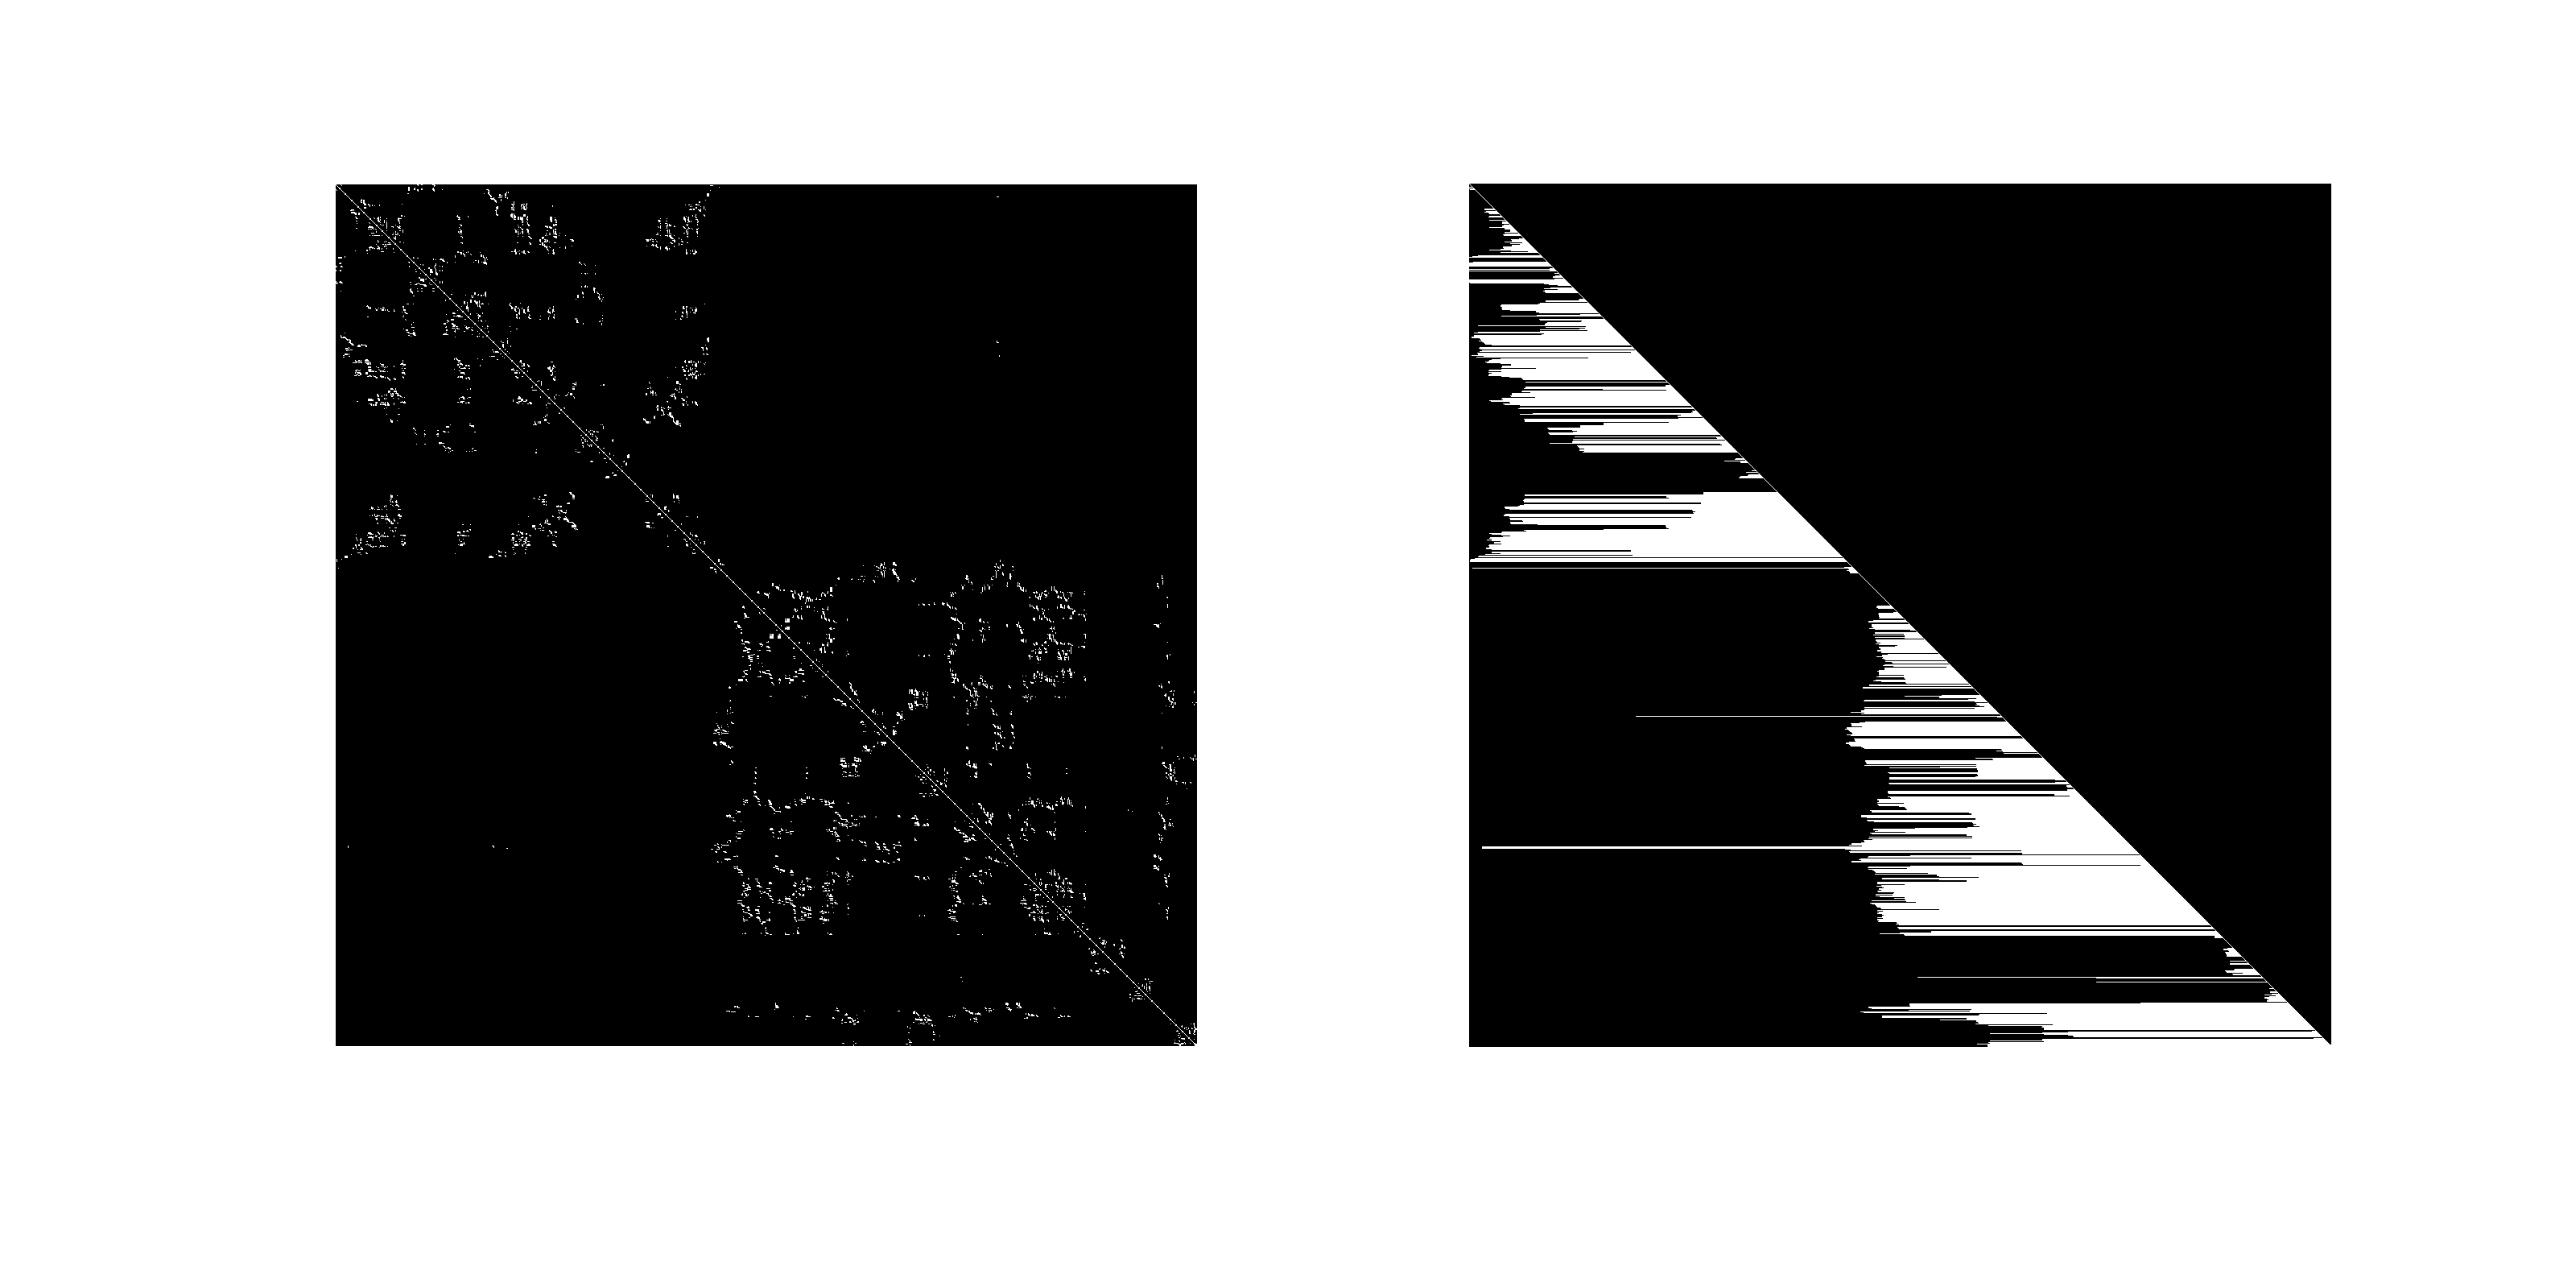
\includegraphics[width=\textwidth]{figures/04_solvingSe3/h_l_no_permutation.pdf}
        \label{fig:cholesky_fill_in_no_odering}
    \end{minipage}\\
    \begin{minipage}[t!]{\textwidth}
        \centering
        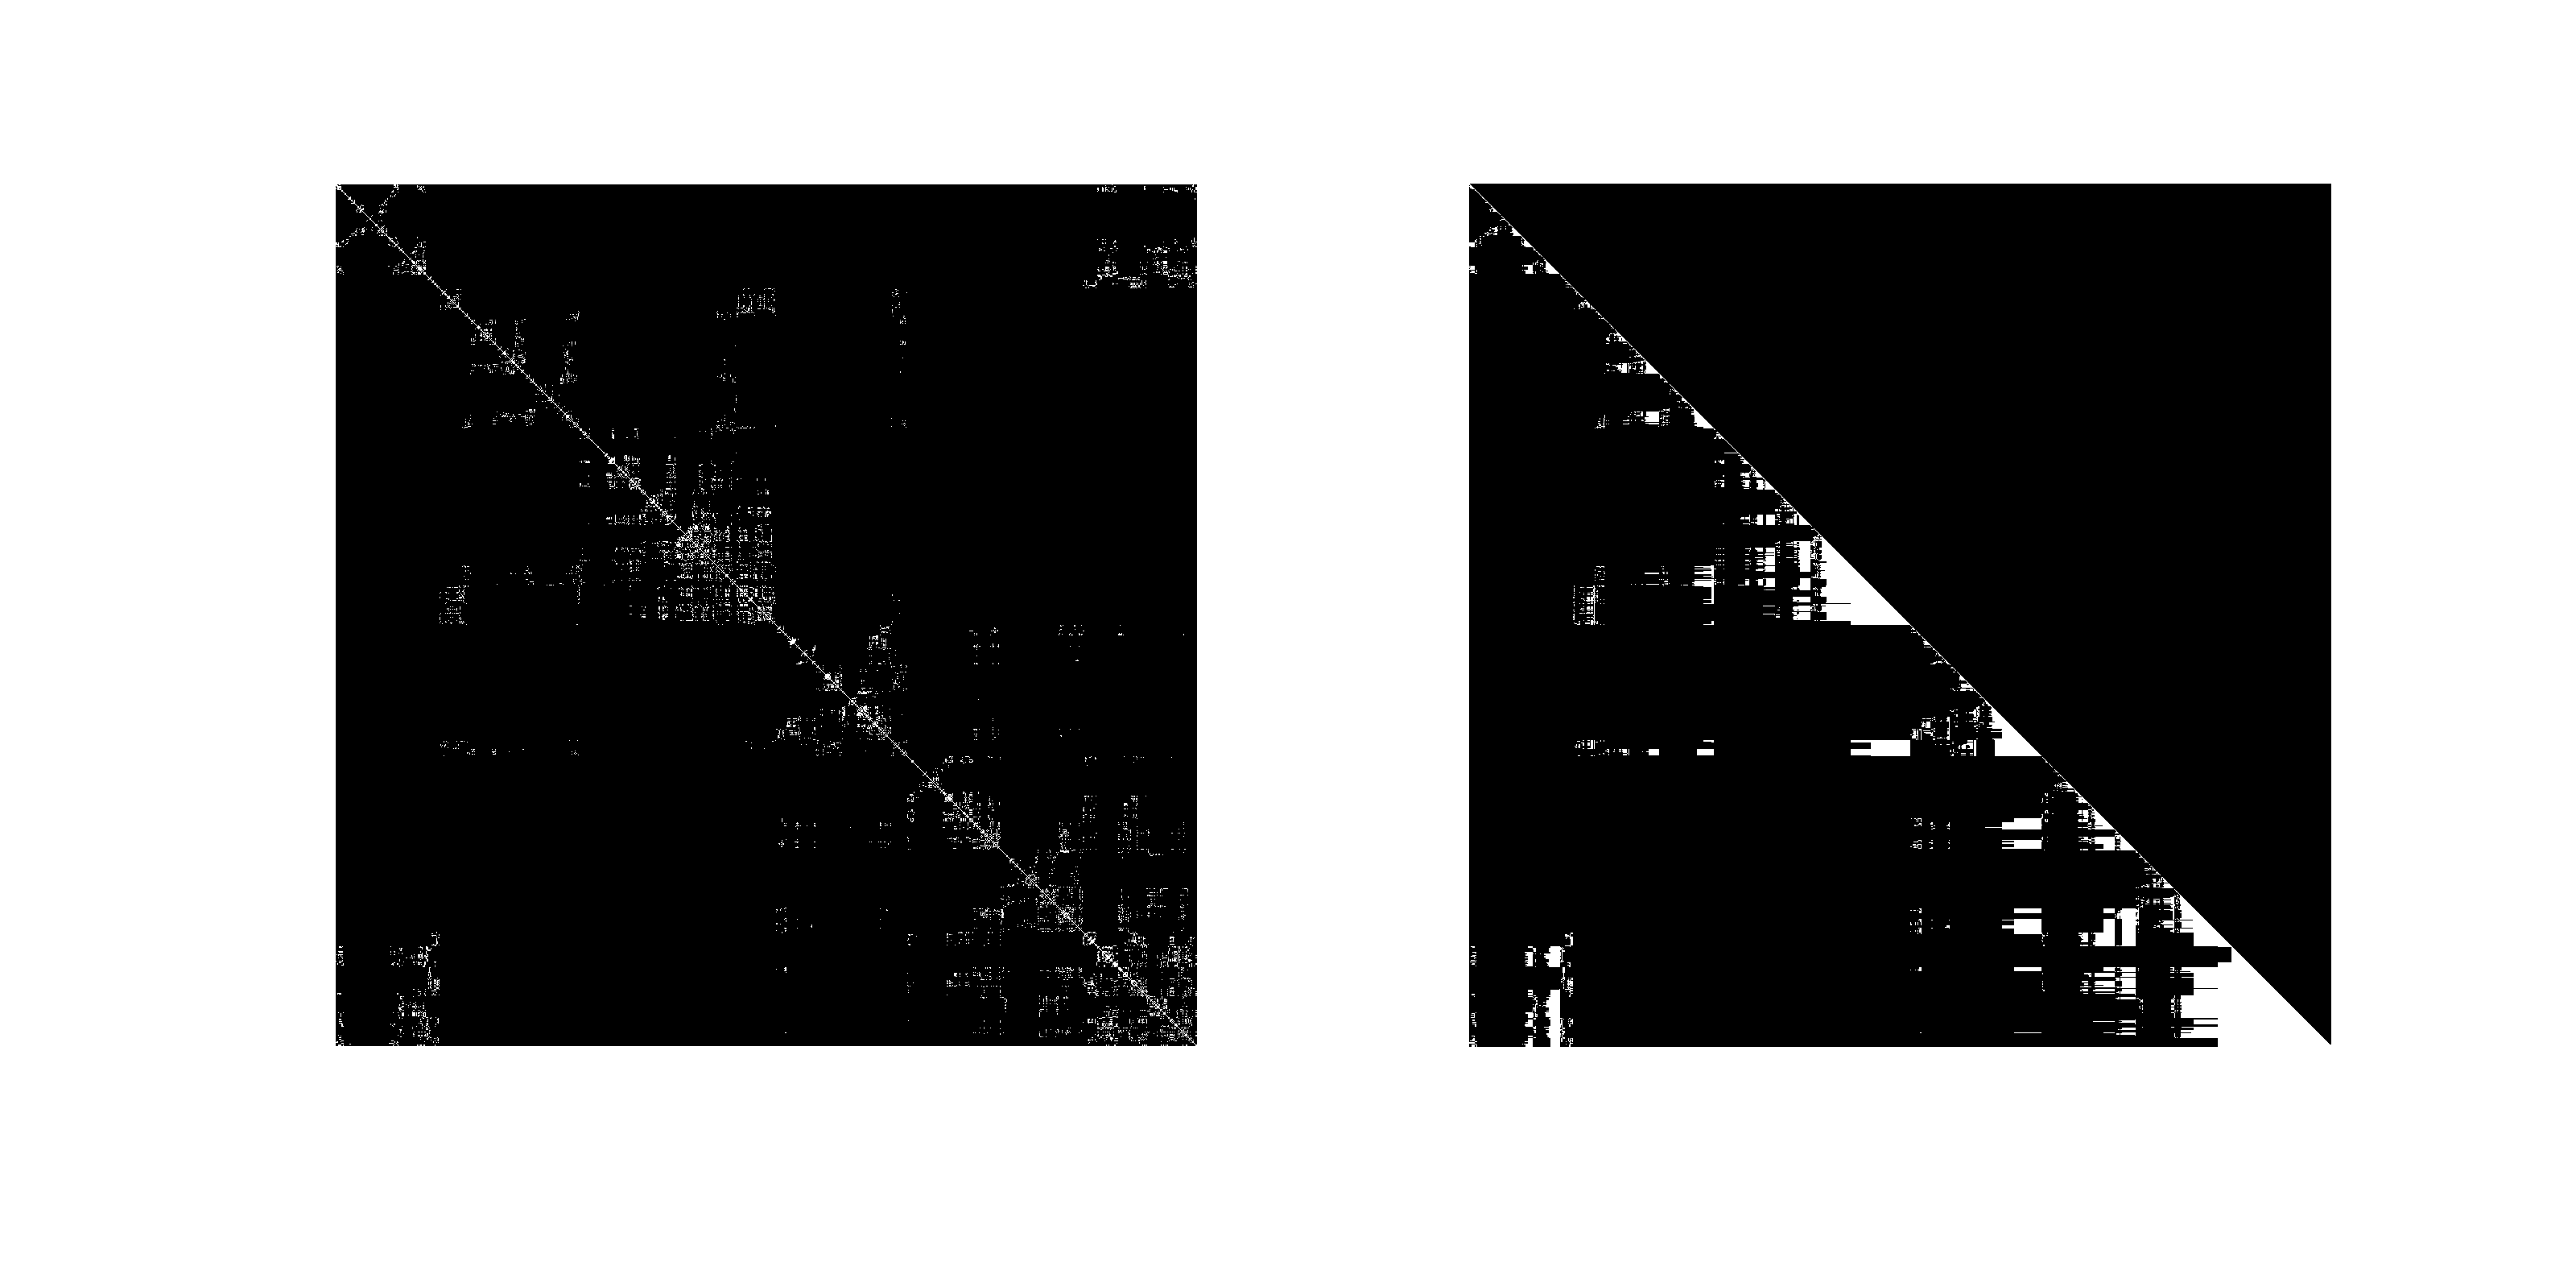
\includegraphics[width=\textwidth]{figures/04_solvingSe3/h_l_amd.pdf}
        \label{fig:cholesky_fill_in_amd}
    \end{minipage}%
    \caption{\textbf{Cholesky Fill-In.} The figure highlights the fill-in due to the factorization of a $(2000\times2000)$ symmetric PSD matrix: non-zero blocks are in white, while null-blocks in black. The first row illustrates the patterns of matrices $\hessian$ and its decomposition $\L$ - respectively on the left and on the right. In the bottom row, the same matrices after the permutation of $\hessian$ using the AMD ordering. It is clear the ordering contribution in reducing the fill-in of the factorization, minimizing the memory required to store $\L$ and the number of block-matrices operations.} 
    \label{fig:cholesky_fill_in}
\end{figure}

As already mentioned in Section \ref{sec:sparse_ls}, variable reordering techniques, that consists in applying a suitable permutation to the source matrix, are able to reduce dramatically the fill-in, allowing a faster decomposition. Several algorithm are proposed in the literature to compute the proper permutation - e.g. AMD, COLAMD. For the Cholesky $LU$ decomposition it is also possible to evaluate the pattern of the $L$ matrix before computing the actual decomposition, through the \textit{Symbolic Cholesky Decomposition}. The reader might appreciate the variable reordering contribution in Figure \ref{fig:cholesky_fill_in}.

In the remaining of the Section, it will be given a more detailed description on how to solve a sparse linear system using the Cholesky decomposition of the matrix $\hessian$.

\subsection{Storage Methods for Sparse Matrices}\label{subsec:sparse_storage_methods}
Another core aspect of sparse matrices is that there are several techniques to \textit{store} them more efficiently, reducing the amount of memory needed. The most general ones are \textit{Compressed Row Storage} (CRS) or \textit{Compressed Column Storage} (CCS), since they do not make any assumption on the structure of the matrix but the do not store unnecessary elements - i.e. the zeros. Those method store the matrix using only 3 vectors: one vector for floating point numbers that represent the non-zero entries and two for the column and row indexes respectively. As an example, given a matrix $A$

\begin{equation*}
    A = 
        \begin{pmatrix}
            10 & 0 & 0 & 0 & -2 & 0 \\
            3 & 9 & 0 & 0 & 0 & 3 \\
            0 & 7 & 8 & 7 & 0 & 0 \\
            3 & 0 & 8 & 7 & 5 & 0 \\
            0 & 8 & 0 & 9 & 9 & 13 \\
            0 & 4 & 0 & 0 & 2 & -1 
        \end{pmatrix}
\end{equation*}

\noindent in CRS format is represented by the following vectors - using zero-based indexing:

\begin{align*}
    val &= \begin{bmatrix}10 & -2 & 3 & 9 & 3 & 7 & \cdots & 2 & -1\end{bmatrix} \\
    col &= \begin{bmatrix}0 & 4 & 0 & 1 & 5 & 1 & \cdots & 4 & 5\end{bmatrix} \\
    row &= \begin{bmatrix}0 & 2 & 5 & 8 & 12 & 16 & 19\end{bmatrix}     
\end{align*}

\noindent \textit{List of Lists} (LIL) represents another effective and easy to implement storage method is the. In this case, each row-vector is represented as a list of pairs that denotes the column index and the element's value.

Recalling equation \ref{eq:sparse_hessian_structure}, since in this problem it has been considered only \textit{binary constraints}, the linearization of each edge generates $4$ block-contributions to the Hessian, namely:

\begin{align*}
    \hessian_{ii} &= \jacob_i^T \Omega_k \, \jacob_i \qquad
    \hessian_{jj} = \jacob_j^T \Omega_k \, \jacob_j \\
    \hessian_{ij} &= \jacob_i^T \Omega_k \, \jacob_j \qquad
    \hessian_{ji} = \jacob_j^T \Omega_k \, \jacob_i 
\end{align*}

\noindent Therefore, the Hessian can be intended to be a \textit{sparse block-matrix} where each entry is a matrix itself of a given size. In our work, it has been chosen to employ the LIL storage method with block-entries, in order to speed-up the numerical computations - better explained in the next Chapter.

\subsection{Cholesky Decomposition}\label{subsec:cholesky_dec_general}
In linear algebra, the Cholesky decomposition (or factorization) is the decomposition of a \textit{Hermitian}, positive semi-definite (PSD) matrix into the product of a \textit{lower triangular matrix} and its \textit{conjugate transpose}, namely

\begin{empheq}[box={\mybluebox[1pt]}]{equation}
    \label{eq:generic_cholesky}
    \mathbf{A} = \L\,\L^\star
\end{empheq}

\noindent In this particular problem formulation, the matrices involved are real, therefore the conjugate transpose of $\L$ is simply its transposed $\L^T = \U$. In this sense, it represents the square-root operator for symmetric PSD matrices.

A more stable variant of the classical Cholesky decomposition is the \textbf{LDL} decomposition. In this case, the original matrix is decomposed into the following product:

\begin{equation}
    \label{eq:ldl_decomposition}
    \mathbf{A} = \L \mathbf{D} \L^\star
\end{equation}

\noindent where $\L$ is a lower \textit{unit} triangular matrix - i.e. all the entries on the main diagonal are $1$ - and $\mathbf{D}$ a diagonal matrix. This variant requires the same space and computational effort with respect to the original one but avoids the square-roots extraction. In this way, even matrices that do not have a Cholesky decomposition can be factorized with the \textit{LDL} one. However, in this work, since the matrix is symmetric and PSD by construction, it has been chose the original Cholesky decomposition.

In general the computational complexity for the factorization of a $(n \times n)$ matrix is $O(n^3)$, requiring about $\nicefrac{n^3}{3}$ FLOPs. There are several algorithm available to compute the factorization, however, one of the most common is the \textit{Cholesky-Banachiewicz}. In this algorithm the computation starts from the top-left corner of the matrix $\L$ and proceeds the computation row-by-row as follows:

\begin{equation*}
    \mathbf{A} = \L \L^T = 
        \begin{pmatrix}
            L_{00} & 0 & 0 \\ L_{10} & L_{11} & 0 \\ L_{20} & L_{12} & L_{22} 
        \end{pmatrix}
        \,
        \begin{pmatrix}
            L_{00} & L_{10} & L_{20} & \\ 0 & L_{11} & L_{21} \\ 0 & 0 & L_{22}
        \end{pmatrix}
\end{equation*}

\noindent where

\begin{empheq}[box={\mybluebox[3pt]}]{equation}
    \label{eq:cholesky_banachiewicz}
    \begin{cases}
        L_{jj} = \sqrt{A_{jj} - \sum_{k = 1}^{j-1}L_{j k}^2} \\
        L_{ij} = \frac{1}{L_{jj}}\left[A_{ij} - \sum_{k = 1}^{j-1}L_{ik}\,L_{jk}\right] \qquad\quad \text{for}\quad i>j
    \end{cases}
\end{empheq}

This algorithm and also the \textit{Cholesky-Crout}'s one - that proceeds column-by-column instead - allow to perform the computation also \textit{in-place}. Moreover, both algorithms can be employed in sparse block-matrices, leading to a block-Cholesky factorization. The blocks are also computed as in Equation \ref{eq:cholesky_banachiewicz} but, in the block case, the \textit{square root} operator is applied to the matrix-block and it consists in the \textit{Cholesky decomposition of the block} itself.

As it has been already mentioned, the main use of the Cholesky decomposition is in the solution of linear systems. Given a symmetric PSD real matrix $\mathbf{A}$, the solution of the linear system $\mathbf{A}\,\state = \bvec$ is computed through the following steps:

\begin{enumerate}
    \item \textbf{Cholesky factorization} of source matrix $\mathbf{A} = \L \L^T$
    \item \textbf{Forward substitution} to solve the linear system $\L \, \mathbf{y} = \bvec$
    \item \textbf{Backward substitution} to solve the linear system $\L^T\, \state = \mathbf{y}$
\end{enumerate}

Clearly, since in the problem in analysis $\hessian$ and its factorization $\L$ are sparse block-matrices, also $\bvec$ and $\mathbf{y}$ are \textit{dense block-vector} - with the number of blocks $N$ equal to the number of vertexes in the graph.

\section{Manifold Representation}\label{sec:manifold_se3}
As it has been already stated at the begin of the Chapter, this work focuses on 3D formulations of pose-graph and bundle adjustment. In this Section it will be better analyzed the representation of all the objects required for the LS estimation in both the formulations.

\subsection{3D Pose-Graph}\label{subsec:3d_pose_graphs}
Pose-graph optimization in 3D represents the backbone of SLAM, allowing to estimate the robot trajectory \textit{in space} through MAP estimation. In this formulation, the state $\state$ includes the 3D orientation of the nodes which represent the main reason why pose-SLAM is a complex problem. Rotations in the space can be over-parametrized through a 3D rotation matrix $\rot \in SO(3)$. Therefore, the over-parametrized state can be represented by a 3D isometry $\SState = \,\T{W}{R} \in SE(3)$ which represents the robot pose in the world reference frame - i.e. a $(4 \times 4)$ homogeneous transformation matrix.

A possible \textit{minimal representation} of the state can be through a $6$ vector $\state = (t_x\,t_y\,t_z\,\alpha\,\beta\,\gamma)^T$, where the triplet $\mathbf{r} = (\alpha\,\beta\,\gamma)^T$ represents the Euler Angles that compose the rotational part of the isometry, while $\trans = (t_x\,t_y\,t_z)^T$ the translational one. Summarizing, in formul\ae:

\begin{equation*}
    \SState = 
        \begin{pmatrix}
            \rot & \trans \\ \zero^T & 1
        \end{pmatrix}
    \qquad 
    \state = \begin{bmatrix} t_x & t_y & t_z & \alpha & \beta & \gamma \end{bmatrix}^T
\end{equation*}

\noindent where

\begin{equation}
    \label{eq:se3_rotation}
    \rot = \rot_x(\alpha) \, \rot_y(\beta)\, \rot_z(\gamma)
\end{equation}

The measurements are also of type \textit{pose}, thus, it is possible to use the same notation that describes the state. Therefore $\Meas_{ij}$ represents the over-parametrized measurement of node $j$ with respect to node $i$ - i.e. a 3D isometry $\T{i}{j}$.

The next required step concerns the definitions of suitable operators \textit{box-plus} and \textit{box-minus}. We introduce again the operators \textit{v2t} and \textit{t2v} that allow to map the over-parametrized representation into the minimal one and vice versa. Those two operators allow to define the following relations:

\begin{align}
    \label{eq:standard_boxplus_se3}
    \SState \boxplus \dx &= \v2t(\dx) \, \SState \\
    \label{eq:standard_boxminus_se3}
    \SState_a \boxminus \SState_b &= \text{t2v}\left(\SState_b^{-1}\SState_a\right)
\end{align}

\noindent For $SE(3)$ object, the \textit{v2t} function computes the rotational part of $\SState$ through Equation \ref{eq:se3_rotation} and then composes the isometry adding the translational part $\trans = (t_x \: t_y \: t_z)^T$. In Equation \ref{eq:se3_rotation} the factors $\rot_x$, $\rot_y$ and $\rot_z$ represent the 3D rotation respectively around the $x$, $y$ and $z$ axis; they are defined as follows:

\begin{align}
    \label{eq:rotx_3d}
    \rot_x(\alpha) &= 
        \begin{bmatrix}
            1 & 0 & 0 \\ 0 & \cos\alpha & -\sin\alpha \\ 0 & \sin\alpha & \cos\alpha
        \end{bmatrix} \\
    \label{eq:roty_3d}
    \rot_y(\beta) &=
        \begin{bmatrix}
            \cos\beta & 0 & \sin\beta \\ 0 & 1 & 0\\ -\sin\beta & 0 & \cos\beta
        \end{bmatrix} \\
    \label{eq:rotz_3d}
    \rot_z(\gamma) &= 
        \begin{bmatrix}
            \cos\gamma & -\sin\gamma & 0 \\ \sin\gamma & \cos\gamma & 0 \\ 0&0&1
        \end{bmatrix} 
\end{align}

Instead, to retrieve the Euler given the rotation matrix $\rot$ - that is done in the \textit{t2v} operator - it is necessary to equate each element in $\rot$ with its corresponding element in the matrix product $\rot_x(\alpha) \, \rot_y(\beta)\, \rot_z(\gamma)$, in formul\ae:

\begin{align}
    \label{eq:rot_composition_xyz}
    \rot &= 
        \begin{bmatrix}
            R_{00} & R_{01} & R_{02} \\
            R_{10} & R_{11} & R_{12} \\
            R_{20} & R_{21} & R_{22} 
        \end{bmatrix}
     = \rot_x(\alpha) \, \rot_y(\beta)\, \rot_z(\gamma) = \\
     &=
        \begin{bmatrix}
            \cos\beta\,\cos\gamma & -\cos\beta\,\sin\gamma & \sin\beta \\
            \cos\alpha\,\sin\gamma + \sin\alpha\,\cos\gamma\,\sin\beta & \cos\alpha\,\cos\gamma - \sin\alpha\,\sin\beta\,\sin\gamma & -\cos\beta\,\sin\alpha \\
            \sin\alpha\,\sin\gamma - \cos\alpha\,\cos\gamma\,\sin\beta & \sin\alpha\,\cos\gamma + \cos\alpha\,\sin\beta\,\sin\gamma & \cos\beta\,\cos\alpha 
        \end{bmatrix} \nonumber
\end{align}

The reader might notice the non-linearities introduced by the functions t2v and v2t. Those imply the computation of complex non-linear derivatives to retrieve the Jacobian in the linearization phase. However, this problem - and the solution proposed in this work - will be better analyzed in the next Section.

\subsection{3D Bundle Adjustment}\label{subsec:3d_bundle_adj}
In this formulation, as already explained in Section \ref{sec:bundle_adjustment_problem}, the system has to estimate both the robot trajectory and the position of salient world points - i.e. the 3D landmarks. Therefore, the system's \textit{state} and \textit{increment} are described as follows:

\begin{align*}
    \SState &= \left(\overbracket{\SState^R_1, ..., \SState^R_N}^{N poses}\: |\: \overbracket{\state^L_{N+1}, ..., \state^L_{N+M}}^{M landmarks}\right) \\
    \dx &= \left(\overbracket{\dx^R_1, ..., \dx^R_N}^{N poses}\: |\: \overbracket{\dx^L_{N+1}, ..., \dx^L_{N+M}}^{M landmarks}\right)
\end{align*}

The formalization for $SE(3)$ nodes remains unchanged from the previous Sub-Section, therefore, it is necessary to characterize only the nodes that describe the landmarks. 

Landmarks' nodes lie on $\mathbb{R}^3$, so it is not necessary to define anything else - i.e. no \textit{box-plus}/\textit{box-minus} operator needed. As a consequence of this, a measurement $\meas_{ij} \in \mathbb{R}^3$ is a simple 3 vector that describes the position of point $j$ in the $i$-th pose reference frame.

However, it is necessary to consider also the fact that the sensor's reference frame and the robot's one might not coincide, but they related through the transformation $\S = \,\T{R}{S} \in SE(3)$. Given this, the \textit{predicted measurement} given the state is:

\begin{equation}
    \label{eq:prediction_se3r3}
    \tmeas_{ij} = h_{ij}(\SState) = \underbracket{\S^{-1}\,\SState_i^{-1}}_{\mathbf{K}}\p_j = \rot_{K}\p_j + \trans_K
\end{equation}

\noindent In light of this, without loss of generality, the error between the predicted and the actual measurement is computed as follows:

\begin{empheq}[box={\mybluebox[0pt]}]{equation}
    \label{eq:error_se3r3}
    \error_{ij} = \tmeas_{ij} - \meas_{ij} = \S^{-1}\SState_i^{-1}\p_j - \meas_{ij}
\end{empheq}

\noindent Given Equation \ref{eq:error_se3r3}, the perturbed error will be:

\begin{equation}
    \label{eq:perturbed_error_se3r3}
    \error_{ij}(\SState_i \boxplus \dx_i^R, \state_j + \dx_j^L) = \S^{-1}\left[\left(\v2t(\dx_i^R)\SState_i\right)^{-1}\left(\p_j+\dx_j^L\right)\right] - \meas_{ij}
\end{equation}

Finally, it is necessary to compute the Jacobian $\jacob$ deriving from the constraint $\meas_{ij}$, that is structured as follows:

\begin{equation*}
    \jacob = \left[\zero \: \cdots \: \zero \:\, \jacob_R \,\: \zero \: \cdots \: \zero \:\, \jacob_L \,\: \zero \: \cdots \: \zero\right]
\end{equation*}

\noindent where

\begin{align*}
    \jacob_R &= \frac{\partial\,\S^{-1} \left[\left(\v2t(\dx_i^R)\SState_i\right)^{-1}\left(\p_j + \dx_j^L\right) - \meas_j\right]}{\partial\dx_i^R} \Bigg \rvert_{\scriptsize\begin{matrix} \dx_i^R = 0\\\dx_j^L = 0\end{matrix}} = \\
    &= \frac{\partial\: \left[\rot_{S}^T\left[\v2t(\dx_i^R) \SState_i\right]^{-1} \, \p_j - \rot_{S}^T\trans_S\right]}{\partial\dx_i^R} \Bigg \rvert_{\scriptsize\begin{matrix} \dx_i^R = 0\\\dx_j^L = 0\end{matrix}} = \\
    &= \frac{\partial\, \rot_{S}^T \SState_i^{-1} \left[\v2t(\dx_i^R)\right]^{-1} \, \p_j}{\partial\dx_i^R} \Bigg \rvert_{\scriptsize\begin{matrix} \dx_i^R = 0\\\dx_j^L = 0\end{matrix}} = \\
    &= \frac{\partial\, \left[\rot_{S}^T\, \rot_{R}^T\, \left[\v2t(\dx_i^R)\right]^{-1} \, \p_j - \rot_{R}^T\,\trans_R\right]}{\partial\dx_i^R}\Bigg \rvert_{\scriptsize\begin{matrix} \dx_i^R = 0\\\dx_j^L = 0\end{matrix}} = \\
    &= \frac{\partial\, \rot_{S}^T \, \rot_{R}^T \left(\left[\v2t(\dx_i^R)\right]^{-1} \, \p_j\right)}{\partial\dx_i^R} \Bigg \rvert_{\tiny\begin{matrix} \dx_i^R = 0\\\dx_j^L = 0\end{matrix}} =
    \rot_{S}^T \, \rot_{R}^T \frac{\partial\, \left[\rot_{\dx_i^R} \,\p_j - \rot_{\dx_i^R} \,\trans_{\dx_i^R}\right]}{\partial\dx_i^R} \Bigg \rvert_{\tiny\begin{matrix} \dx_i^R = 0\\\dx_j^L = 0\end{matrix}} 
\end{align*}

\noindent Exploiting the fact that the derivative expressed in the previous equation is evaluated in $\dx_i^R = 0$, it leads to the following relation:

\begin{empheq}[box={\mybluebox[0pt]}]{equation}
    \label{eq:jac_r_se3r3}
    \jacob_R = \rot_{S}^T \: \rot_{R}^T \: \begin{bmatrix} -I_{3\times3} & | & -{\lfloor\p_j\rfloor}_\times\,\end{bmatrix}
\end{empheq}

\noindent The other component of $\jacob$ - namely $\jacob_L$ - instead can be computed as follows:

\begin{align*}
    \jacob_L &= \frac{\partial\,\S^{-1} \left[\left(\v2t(\dx_i^R)\SState_i\right)^{-1}\left(\p_j + \dx_j^L\right) - \meas_j\right]}{\partial\dx_j^L} \Bigg \rvert_{\scriptsize\begin{matrix} \dx_i^R = 0\\\dx_j^L = 0\end{matrix}} = \\
    &= \frac{\partial\,\left[\rot_{S}^T \, \SState_i^{-1}\left(\p_j + \dx_j^L\right) - \rot_{S}^T \, \trans_S\right]}{\partial\dx_j^L} \Bigg \rvert_{\scriptsize\begin{matrix} \dx_i^R = 0\\\dx_j^L = 0\end{matrix}} = \\
    &= \frac{\partial\,\left[\left(\rot_{S}^T \, \SState_i^{-1}\p_j\right) +  \left(\rot_{S}^T \, \SState_i^{-1}\dx_j^L\right)\right]}{\partial\dx_j^L} \Bigg \rvert_{\scriptsize\begin{matrix} \dx_i^R = 0\\\dx_j^L = 0\end{matrix}} = 
    \rot_{S}^T \, \frac{\partial\,\left[\rot_R^T \, \dx_j^L  - \rot_{R}^T\trans_R\right]}{\partial\dx_j^L} \Bigg \rvert_{\scriptsize\begin{matrix} \dx_i^R = 0\\\dx_j^L = 0\end{matrix}} 
\end{align*}

%\dx_i^R = 0, \dx_j^L = 0

\noindent This result - expanding the derivatives and exploiting that the linearization point is $\dx_j^L = 0$ - leads to the following relation:

\begin{empheq}[box={\mybluebox[0pt]}]{equation}
    \label{eq:jac_l_se3r3}
    \jacob_L = \rot_{S}^T\:\rot_{R}^T
\end{empheq}

\noindent The reader might notice that $\jacob_R$ is a $(3 \times 6)$ matrix - since the minimal representation of $SE(3)$ states has $6$ components - while $\jacob_L$ is a $(3\times3)$ matrix - because $\mathbb{R}^3$ states are vectors with only $3$ components. 

\vspace{15px}

In the next Section it is proposed a deeper analysis on the error representation and the linearization of 3D pose constraints, highlighting the non-linearity of the computation and the proposed approach to overcome this issue.

\section{Dealing with SE3 Objects}{\label{sec:se3_objects}}
3D poses are complex objects to manage, due to their rotational part that introduces many an highly non-linear contribution in the linearization process. In this section it is proposed an approach that aims to reduce those non-linearities while delivering performances comparable to other state-of-the-art systems.

\subsection{Chordal Distance Based Error Function}\label{subsec:chordal_dist_error}
Recalling \ref{subsec:3d_pose_graphs}, we have defined the functions v2t and t2v that allow to map the minimal representation of the state into the redundant one and vice-versa. Through them, we defined the operators \textit{box-plus} and \textit{box-minus}, described respectively in Equations \ref{eq:standard_boxplus_se3} and \ref{eq:standard_boxminus_se3}. Sticking to this notion, the \textit{predicted measurement} $\Pred_{ij}$ of pose $j$ from pose $i$ is computed as

\begin{equation}
    \label{eq:standard_prediction_se3}
    \Pred_{ij} = h_{ij}(\SState) = \SState_i^{-1}\SState_j
\end{equation}

\noindent that leads to the following error function:

\begin{equation}
    \label{eq:standard_error_se3}
    \error_{ij}(\SState) = \Pred_{ij} \boxminus \Meas_{ij} = \text{t2v}\left(\Meas_{ij}^{-1}\: \SState_i^{-1} \: \SState_j\right)
\end{equation}

\noindent The error $\error_{ij}$ is a 6 vector that expresses the mismatch of each component of state's minimal representation. Proceeding with the error perturbation, the result will be:

\begin{equation}
    \label{eq:standard_perturbated_error_se3}
    \error_{ij}(\SState_i \boxplus \dx_i, \SState_j \boxplus \dx_j) = \text{t2v}\left(\Meas_{ij}^{-1}\left(\v2t(\dx_i)\,\SState_i\right)^{-1} \, \left(\v2t(\dx_j)\,\SState_j\right)\right)
\end{equation}

The full Jacobian $\jacob = \left[\zero \: \cdots \: \zero \:\, \jacob_i \,\: \zero \: \cdots \: \zero \:\, \jacob_j \,\: \zero \: \cdots \: \zero\right]$  will be quite complex to compute due to the derivative of the t2v and v2t functions, requiring also many FLOPs and, thus, slowing the optimization process. In this formulation $\jacob_i$ and $\jacob_j$ are $(6\times6)$ matrices.

It is possible to approach this problem using a different error formulation that leads to easy-to-compute derivatives. In order to do so, we define the $L_{p,q}$ norm of a $(m\times n)$ matrix $A$ as follows:

\begin{equation*}
    \norm{A}_{p,q} = \left(\sum_{j=1}^{n} \left(\sum_{i=1}^{m} |a_{ij}|^p \right)^{\nicefrac{q}{p}}\right)^{\nicefrac{1}{q}}
\end{equation*}

\noindent For $p = q = 2$ the becomes

\begin{empheq}[box={\mybluebox[2pt]}]{equation}
    \label{eq:frobenius_norm}
    \norm{A}_F = \left( \sum_{j=1}^{n} \left(\sum_{i=1}^{m}|a_{ij}|^2 \right)^{\nicefrac{2}{2}}\right)^{\nicefrac{1}{2}} = \sqrt{\sum_{i=1}^{m}\:\sum_{j=1}^{n}|a_{ij}|^2}
\end{empheq}

\noindent that represents the \textit{Frobenius norm} of a matrix, an \textit{entrywise} norm, which is also \textit{invariant under rotation} constraint. Based on this concept, it is possible to define the \textit{chordal distance} between two rotation matrix $\rot_{A}$ and $\rot_{B}$ as follows:

\begin{equation}
    \label{eq:chordal_distance_true}
    d_{\text{chord}}(\rot_{A}, \rot_{B}) = \norm{\rot_{A} - \rot_{B}}_F
\end{equation}

\noindent It is good to notice that the difference operator employed in Equation \ref{eq:chordal_distance_true} is the standard Euclidean \textit{minus}, executed element-wise.

\begin{figure}[!hbt]
    \centering
    \resizebox{0.7\textwidth}{!}{\input{figures/04_solvingSe3/chordal_distance.pdf_tex}}
    \caption{\textbf{Chordal Distance.} This figure shows the underlying concept of the new error function: the distance between $\mathbf{p}_1$ and $\mathbf{p}_2$ can be approximated with the Euclidean distance computed between the projection of those points onto the relative chord - namely between $\hat{\mathbf{p}}_1$ and $\hat{\mathbf{p}}_2$.} 
    \label{fig:chordal_distance}
\end{figure}

We define also a new function, that given a 3D isometry returns a 12 vector made with its components, namely:

\begin{align}
    \SState &= 
        \begin{bmatrix}
            \rot & \trans \\ \zero & 1
        \end{bmatrix} \nonumber \\
    \rot &= \begin{pmatrix} \mathbf{r}_1 | \mathbf{r}_2 | \mathbf{r}_3 \end{pmatrix} \nonumber \\
    \text{flatten}(\SState) &= \begin{pmatrix} \mathbf{r}_1 \\ \mathbf{r}_2 \\ \mathbf{r}_3 \\ \trans \end{pmatrix}
    \label{eq:flatten_isometry_operator}
\end{align}

\noindent where $\mathbf{r}_k$ represents the $k$-th column of $\rot$.

Finally, we introduce the following relations to express operators \textit{box-plus} and \textit{box-minus}:

\begin{align}
    \label{eq:boxplus_se3}
    \SState \boxplus \dx &= \v2t(\dx)\, \SState \\
    \label{eq:boximus_se3}
    \SState_a \boxminus \SState_b &= \flatten{\SState_a} - \flatten{\SState_b}
\end{align}

Given those mathematical concepts, it is possible to define the error between two $SE(3)$ objects through a relaxed version of the chordal distance, that leads to the following relations:

\begin{align}
    \label{eq:prediction_se3}
    \Pred_{ij} = h_{ij}(\SState) &= \flatten{\SState_i^{-1}\,\SState_j} \\
    \label{eq:error_se3}
    \error_{ij}(\SState) = \Pred_{ij} - \Meas_{ij} &= \flatten{\SState_i^{-1}\, \SState_j} - \flatten{\Meas_{ij}}
\end{align}

\noindent It is good to notice that $\error_{ij}$ now is a 12 vector, therefore, the Jacobian's components $\jacob_i$ and $\jacob_j$ will be $(12\times6)$ matrices. Speaking of this, applying the state perturbation to the error will lead to the following relation:

\begin{equation}
    \label{eq:perturbed_error_se3}
    \error_{ij}(\SState_i \boxplus \dx_i, \SState_j \boxplus \dx_j) = \flatten{\left(\v2t(\dx_i)\SState_i\right)^{-1}\,\left(\v2t(\dx_j)\SState_j\right)} - \flatten{\Meas_{ij}}
\end{equation}

\noindent It is already possible to notice the reduced complexity of the derivatives required to linearize the constraint. In fact, from Equation \ref{eq:perturbed_error_se3} it is possible to retrieve the following relations - stating that $\rot_{\dx_i} = \rot_{\dx_i}^x \, \rot_{\dx_i}^y \, \rot_{\dx_i}^z$:

\begin{align*}
    \jacob_j &= \frac{\partial\: \error_{ij}(\SState_i \boxplus \dx_i, \SState_j \boxplus \dx_j)}{\partial \dx_j} \Bigg \rvert_{\scriptsize\begin{matrix} \dx_i = 0\\\dx_j = 0\end{matrix}} = \\
    &= \frac{\partial \left[\flatten{\overbracket{\begin{bmatrix}\rot_i^T & -\rot_i^T \trans_i \\\zero & 1\end{bmatrix} \begin{bmatrix}\left(\rot_{\dx_i}^x \, \rot_{\dx_i}^y \, \rot_{\dx_i}^z\right)^T & -\rot_{\dx_i}^T \trans_i \\\zero & 1\end{bmatrix} \begin{bmatrix}\rot_j & \trans_j \\\zero & 1\end{bmatrix}}^{\mathbf{G}}}\right]}{\partial \dx_j} \Bigg \rvert_{\scriptsize\begin{matrix} \dx_i = 0\\\dx_j = 0\end{matrix}} 
\end{align*}

\noindent Expanding the derivatives, it is possible to define the following - intuitively retrieved - objects:

\begin{itemize}
    \item  $\rot_{x0}^{\prime}$, $\rot_{y0}^{\prime}$ and $\rot_{z0}^{\prime}$ that represent derivative with respect to $\Delta\alpha$, $\Delta\beta$ and $\Delta\gamma$ of the base rotation $\rot_k(\cdot)$, evaluated in 0 and with $k = \{x,y,z\}$.
    \item  $\hat{\rot}_{x0}^{\prime}$, $\hat{\rot}_{y0}^{\prime}$, and $\hat{\rot}_{z0}^{\prime}$ that are the derivative with respect to $\Delta\alpha$, $\Delta\beta$ and $\Delta\gamma$ of the rotational part of matrix $\mathbf{G}$, computed as $\hat{\rot}_{k0}^{\prime} = \rot_{i}^T \, \rot_{k0}^{\prime} \, \rot_j$ with $k = \{x,y,z\}$
    \item $\hat{\mathbf{r}}_{k0}^{\prime}$ which describes the 9 vector obtained stacking the columns of $\hat{\rot}_{k0}^{\prime}$ - with $k = \{x,y,z\}$
\end{itemize}

\noindent In the light of what we just stated, it is possible to retrieve this final formulation of $\jacob_j$:

\begin{empheq}[box={\mybluebox[3pt]}]{equation}
    \label{eq:jac_j_se3} 
    \jacob_j = 
        \begin{pmatrix}
            \zero_{(9\times3)} & \begin{bmatrix} \hat{\mathbf{r}}_{x0}^{\prime} & | & \hat{\mathbf{r}}_{y0}^{\prime} & | & \hat{\mathbf{r}}_{z0}^{\prime} \end{bmatrix}_{(9\times3)} \\
            \rot_{i}^T & -\rot_{i}^T \, \skew{\trans_j}
        \end{pmatrix}
\end{empheq}

\noindent Intuitively, the other component of the Jacobian will be simply

\begin{empheq}[box={\mybluebox[3pt]}]{equation}
    \label{eq:jac_i_se3}
    \jacob_i = -\jacob_j
\end{empheq} 

The reader might noticed how the new error function reduced the computational cost of the derivatives, due to the elimination of the highly non-linear function t2v. Moreover, the use of standard Euclidean \textit{minus} operator to express differences between transforms, leads to a better approximation by the first-order Taylor expansion of the perturbed error. This better approximation, translates into a wider converge basin of the optimization process and into an improved the avoidance of local minima.

\subsection{Benefits in the Re-linearization}\label{subsec:benefits}
The reader might remember that, since also the measurements live on a non-Euclidean space, it is necessary to project the measurement information matrices through the \textit{box-minus} operator. Therefore, using the standard \textit{box-minus} described in Equation \ref{eq:standard_boxminus_se3} and given $\Pred_{ij}$ associated to $\Meas_{ij} = \Meas_{k}$, it is required to compute the following objects \textbf{at each iteration} of the LS optimization:

\begin{align}
    \label{eq:jacobian_meas_se3}
    \jacob_{\Meas_{k}} &= \frac{\partial \left(\Pred_{ij} \boxminus \Meas\right)}{\partial \Meas} \bigg\rvert_{\Meas = \Meas_{k}} \\
    \label{eq:std_adapted_information_matrix_se3}
    \tilde{\Omega}_k &= \left(\jacob_{\Meas_{k}} \: \Omega_k \: \jacob_{\Meas_{k}}^T\right)^{-1}
\end{align}

The error function based on the chordal distance that it has been proposed in the previous Sub-section, brings benefits also in this sense. In fact, since the operator employed to compute the error is the standard Euclidean \textit{minus}, it is not required to recompute the information matrix $\Omega_k$ at each iteration. 

It is good to notice that the information matrix associated with the measurement $\Meas_{k}$ is a $(6\times6)$ matrix $\Omega_k$ , since the state's minimal representation has dimension $6$ in this formalization. However, it is necessary to consider the contribute of function $\flatten{\cdot}$ in this process: the new error space has dimension $12$, thus it is necessary to project the information matrix into the new higher dimensional space. To this end, will now propose some new mathematical concepts useful in order to estimate the result of applying a non-linear transformation to a probability distribution function. 

Given a Gaussian distribution $p(x) = \mathcal{N}(x; \mu, \Sigma)$ with mean $\mu$ and covariance $\Sigma$, it is possible to represent it through a set of weighted points called \textit{Sigma Points}. Each Sigma Point $\chi^i$ is described by a set of parameters:

\begin{itemize}
    \item a \textbf{position} $x^i$
    \item a \textbf{weight for the mean} $w_m^i \in \mathbb{R}^+$
    \item a \textbf{weight for the covariance} $w_c^i \in \mathbb{R}^+$
\end{itemize}

\noindent Clearly, the conversion from the original parameters $(\mu, \Sigma)$ to the Sigma Points $\chi^i = (x^i, w_m^i, w_c^i)$ must be invertible. In fact, it is possible to reconstruct the Gaussian parameters from the Sigma Points as follows:

\begin{align}
    \label{eq:sigma_to_mean}
    \mu &= \sum_i w_m^i \: x^i \\ 
    \label{eq:sigma_to_covariance}
    \Sigma &= \sum_i w_c^i\:(x^i - \mu)(x^i - \mu)^T
\end{align}

It is good to notice that, if the original Gaussian distribution has dimension $n$, a suitable number of Sigma Point required to approximate without loosing information will be $N = 2n + 1$. In order to control how far the Sigma Points are sampled from the mean $\mu$ though, it is possible to tune the scalar parameters $\kappa \in \mathbb{R}^+$ and $\alpha \in (0,1]$. Therefore, the position of each Sigma Point is computed as follows:
\begin{align}
    \label{eq:sigma_point_pos_0}
    x^{(0)} &= \mu \\
    \label{eq:sigma_point_pos_i}
    x^{(i)} &= 
    \begin{cases}
        \mu + [L]_i \qquad \quad \text{for} \: i \in [1 \dots n] \\
        \mu - [L]_{n-i} \qquad \text{for} \: i \in [n+1 \dots 2n]
    \end{cases}
\end{align}

\noindent where $L = \sqrt{(n + \lambda)\Sigma}$ and $\lambda = \alpha^2 (n + \kappa) - n$. Given the scalar parameter $\beta = 2$ - tuned for Gaussian PDFs - the weights are retrieved as follows:

\begin{align}
    \label{eq:sigma_point_wm_0}
    w_m^{(0)} &= \frac{\lambda}{\lambda + n} \\
    \label{eq:sigma_point_wc_0}
    w_c^{(0)} &= w_m^{(0)} + (1 - \alpha^2 + \beta) \\
    \label{eq:sigma_point_weights_i}
    w_c^{(i)} = w_m^{(i)} &= \frac{1}{2(n + \lambda)}
\end{align}

This transformation between actual Gaussian parameters and the Sigma Points is called \textbf{Unscented Transform} \cite{julier2002scaledUT}. The core feature of this mathematical function is that it can be used to apply a transformation to a PDF in very straightforward way. Sticking to Gaussian PDFs, given $X_a \sim \mathcal{N}(x_a; \mu_a, \Sigma_a)$ and its Unscented Transform $x_a \sim \mathcal{UT}(x_a; x_a^{(i)}, w_m^{(i)}, w_c^{(i)})$, computing the Gaussian $X_b = g(X_a)$ can require a lot of effort. However, a good approximation of $X_b$ can be computed applying the function $g(\cdot)$ to the Unscented Transformation of $X_a$. This translates in the application of the $g(\cdot)$ function to each Sigma Point of $x_a$, namely

\begin{empheq}[box={\mybluebox[3pt]}]{equation}
    \label{eq:pdf_function_UT}
    \chi_b^{(i)} = g\left(\chi_a^{(i)}\right) \qquad i = 1 \dots N
\end{empheq}

Going back to our problem, it is possible to transform the information matrix of each measurement $\Omega_k$ through the Unscented Transform. The required steps are the following:

\begin{enumerate}
    \item Compute the $N = 2n+1$ Sigma Points $\chi_{original}^{(i)} = (x_{original}^{(i)}, w_m^{(i)}, w_c^{(i)})$ from $\mathcal{N}(\mu_k, \Sigma_k)$, where $n$ is the minimal representation's dimension (in this case $n = 6$), $\mu_k = \text{t2v}(\Meas_{k})$ and $\Sigma_k = \Omega_k^{-1}$.
    \item Compute the new position of $\chi_{transformed}^{(i)}$ as $x_{transformed}^{(i)} = \flatten{\v2t(x_{original}^{(i)})}$
    \item Reconstruct the new Gaussian $\mathcal{N}(\bar{\mu}_k, \bar{\Sigma}_k)$ from the Sigma Points $\chi_{transformed}^{(i)}$, leaving the parameters $w_m^{(i)}$ and $w_c^{(i)}$ unchanged.
\end{enumerate}

The adapted information matrix $\bar{\Omega}_k = \bar{\Sigma}_k^{-1}$ is a $(12\times12)$ matrix. However, since we are mapping a 6-dimensional space in a 12-dimensional space with only $N = 2n + 1 = 13$ Sigma Points, it is possible to retrieve covariance matrix subject to (multiple) rank-loss. Therefore, it is necessary to add a non-zero scalar $\epsilon$ to the main diagonal of $\bar{\Sigma}_k$, in order to do not have numerical problems during its inversion.

Thanks to the Unscented Transform it is possible to have a fast and quite accurate approximation of the adapted information matrix, leading to consistent results from the optimization process. Moreover, since the minus operator employed in this formulation is the standard Euclidean one, the computation is performed just one time for each measurement $\Meas_{k}$, reducing the computational effort of each optimization step.

\vspace{15px}

All those features lead to an accurate and fast optimizer, that delivers results comparable to other state-of-the-art systems. In the next Chapter, the reader will have an insight on the actual implementation of the system, in order to better understand how all those mathematical concepts have been applied in practice.
\newpage
\chapter{Implementing a Sparse Solver}\label{ch:spsolver}
\lipsum

\lipsum

\newpage
\chapter{Use Cases}\label{ch:cases}
As already mentioned, the system developed aims to deliver real time performances also when used in real world applications. Furthermore, the system provides some easy-to-embed APIs in order to be easily integrated in a full SLAM pipeline. Therefore, in this Chapter we provide two front-end systems developed in the Lab-Rococo at Sapienza University that actually use this work as back-end. In both cases, our system is used to perform 3D \textit{pose-graph} optimization.

\section{ProSLAM}\label{sec:proslam}
The work of Schlegel \textit{et al.} \cite{schlegel2017proslam} presents a stereo visual system capable of mapping dynamic large-scale environments called ProSLAM. The system is designed with simplicity and modularity in mind and, thus, it is easy to implement and to understand also from people who are not Computer Vision or SLAM experts.

This works is also almost entirely self-contained and employs only a minimal set of external libraries - among which there is the library described in this work.

ProSLAM, despite its simplicity, is able to provide results comparable with other more complex state-of-the-art front-ends. Its goal is to generate a 3D map from the processing of a sequence of stereo-images. The map is intended as a collection of \textit{landmarks} - salient 3D points in the world characterized in its appearances by a unique descriptor - together with the camera trajectory. 

Landmarks acquired in a nearby region define a \textit{local-map}, and each of them constitutes a node of the graph - i.e. a $SE(3)$ transformation matrix. Edges between local maps encode the spatial constraints correlating local maps close in space. Those constraints are generated by two kind of events:

\begin{enumerate}
    \item \textbf{Tracking} of the camera motion between temporal subsequent maps
    \item \textbf{Alignment} of local maps acquired at distant times as a consequence of \textit{re-localization} events - i.e. \textit{loop-closures}.
\end{enumerate}

Re-localization is more complex to address with respect to tracking. In fact, to achieve this goal it is necessary to compare descriptors of all the local-maps. This is an expensive operation, and it is efficiently performed by the \textit{Hamming Binary Search Tree} (HBST) \cite{schlegel2016hbst} library. The system periodically triggers graph optimization and this helps also the re-localization process.

It is good to notice that ProSLAM runs on \textit{single thread}, delivering performances comparable with other more complex and multi-thread systems - e.g. \cite{mur2017orb-slam2}.

TODO results

\section{ProSLAM-stud}\label{sec:froslam}
Colosi \textit{et al.} propose in their work ProSLAM-stud \cite{colosi2017froslam} a further iteration on minimalism from original ProSLAM. It is a \textit{Master thesis} work, therefore its approach is more didactic than the original one. However, the system still delivers quite good performances both in terms of speed and accuracy. 

This systems embeds a new \textit{tracking} method based on KD-Tree, that improves the \textit{open-loop estimation} and is able to provide a boost in speed with respect to ProSLAM. 

Having a good open-loop estimate translates into a better initial guess of the optimization problem and, therefore, the whole system can benefit of this novelty. ProSLAM-stud keeps the single-treaded implementation and despite the minimal approach, it can push up to more than 80Hz - on average.

TODO results
\newpage
\chapter{Conclusions}\label{ch:conclusions}
\lipsum

\newpage
\bibliographystyle{splncs}
\bibliography{references}


%add appendix for dataset class
\end{document}